\documentclass{beamer}

% Use a modern, clean theme
\usetheme{metropolis}

\usepackage[utf8]{inputenc}
\usepackage{graphicx}
\usepackage{tikz}
\usepackage{lmodern}


% Title and author info
\title[AI Integration in Education and Dev]{Integration of Artificial Intelligence in Education and Software Development}
\author[Luna Schätzle \& Florian Prandstetter]{Luna Schätzle \\ Florian Prandstetter}
\institute[HTL Anichstraße]{HTL Anichstraße, Department of Business Informatics\\Thesis Supervisor: \\Mag. Dr. Dipl.-Ing. Albert Greinöcker\\MMag.\textsuperscript{a} Eva-Maria Egger, MA}
\date{Diploma Thesis Defense -- April 2025}

% Logo placed at the top-right
\logo{
\includegraphics[height=1cm]{HTL-logo.jpeg}}

% Optional background watermark for additional visual appeal
%\setbeamertemplate{background}{%
%  \begin{tikzpicture}[remember picture,overlay]
%    \node[opacity=0.1, at=(current page.center)] 
%      {
\includegraphics[width=0.5\textwidth]{HTL-logo.jpeg}};
%  \end{tikzpicture}
%}

\begin{document}

\begin{frame}
  \maketitle
\end{frame}



\begin{frame}{Introduction}
  \begin{columns}
    \column{0.75\textwidth}
      \begin{itemize}
        \item \textbf{Presenter:} Florian Prandstetter 
        \item \textbf{Objective:} Server, VS Code Extension \& Operating Systems
        \item \textbf{Focus:} Develop an open-source Extension for Visual Studio Code and a stable server enviorment
      \end{itemize}
    \column{0.25\textwidth}
      \centering
  \end{columns}
\end{frame}



\begin{frame}{Server}
  \begin{itemize}
    \item \textbf{Server Hardware:}
    %Bild???
      \begin{itemize}
        \item CPU: Intel Core i5.8600k
        \item GPU: NVIDA GeForce RTX 2060
        \item RAM: 16GB DDR4 
        \item Motherboard: H370 Chipset
        \item Power Supply: 500W BeQuiet
        \item Storage: 512GB NVMe SSDd
      \end{itemize}
    \item \textbf{Networking:}
      \begin{itemize}
        \item Axios: Used for server requests 
        \item Tailscale: VPN tunnel used for secure remote access 
      \end{itemize}
    \item \textbf{Backup and Recovery:} Regular system backups have been made to avoid data loss.      
  \end{itemize}
\end{frame}

\begin{frame}{Operating System}
  \begin{columns}
    \column{0.5\textwidth}
      \begin{itemize}
        \item \textbf{Used Operating System:} The Server is running with the Ubuntu Server Operating System. 
        \begin{itemize}
          \item Good basis for AI models
          \item CUDA support
        \end{itemize}
      \end{itemize}
    \column{0.5\textwidth}
      \centering
      
\includegraphics[width=0.5\textwidth]{Ubuntu.png}
  \end{columns}

\end{frame}


\begin{frame}{Operating System Market Share} 
  \begin{columns}
    \column{0.5\textwidth}
      \textbf{For Personal Use}
      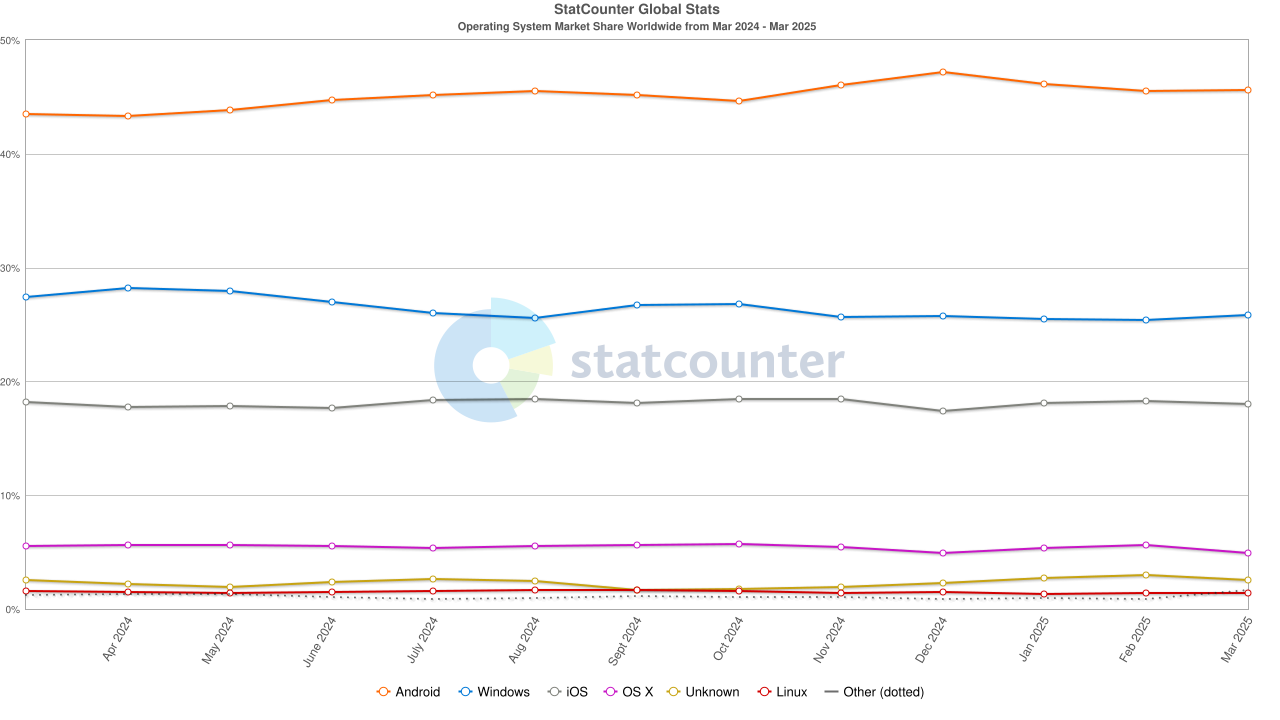
\includegraphics[width=\textwidth]{StatCounter.png}
    \column{0.5\textwidth}
      \textbf{For Servers}
      
      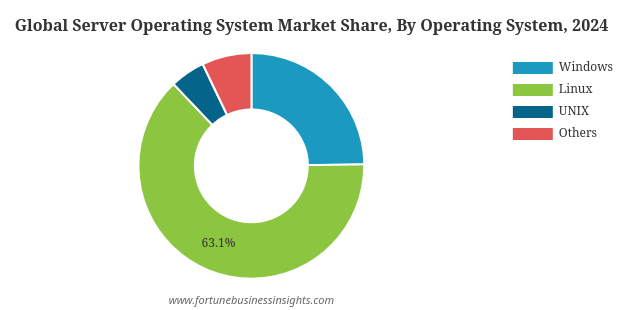
\includegraphics[width=\textwidth]{ServerOSShare.png}
  \end{columns}
\end{frame}

\begin{frame}{Server Operating System Market Volume} 
  \begin{itemize}
    \item Glabal Market Share: America 59,56\text{\%}
    \item CAGR: 12,4\text{\%}
    \item Expected to double by 2032
    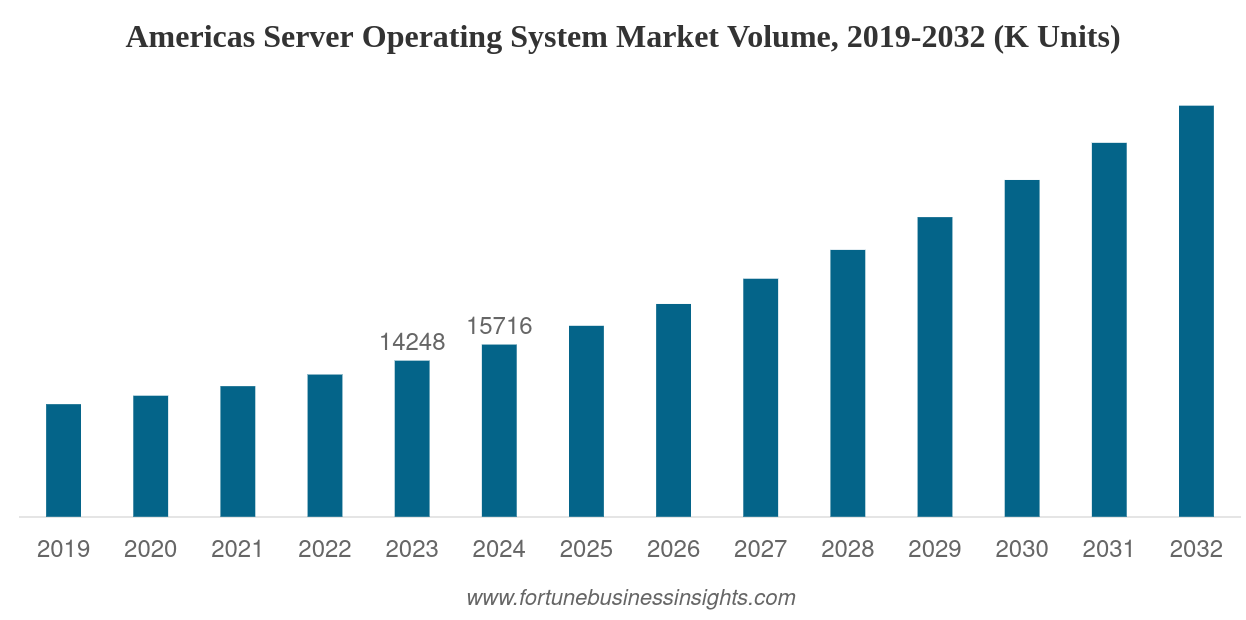
\includegraphics[width=0.8\textwidth]{Server-Market-Volume.png}
  \end{itemize}
\end{frame}


\begin{frame}{Flask Service}
  \begin{itemize}
    \item \textbf{Restful Endpoints and Functionalities:}
    \begin{itemize}
      \item Chatbot 
      \item Programming bot
      \item Obtical Character Recognition 
    \end{itemize}
    \item \textbf{Deployment with Docker:}
    \begin{itemize}
      \item Dockerfile
      \item Docker-Compose
    \end{itemize}
  \end{itemize}
\end{frame}

\begin{frame}{Flask Service}
  \begin{itemize}
    \item Architecture and Service Structure
    \includegraphics[width=\textwidth]{flask_service.png}
  \end{itemize}
\end{frame}



\begin{frame}{Visual Studio Code Extension}
  \begin{columns}
    \column{0.5\textwidth}
      \begin{itemize}
        \item \textbf{Integrated AI Chatbot}
        \item \textbf{Technologies:}
        \begin{itemize}
          \item VS Code API
          \item Type Script
        \end{itemize}
        \item \textbf{Server Requests:}  Are handled with Axios to create a stable connection.
      \end{itemize}
    \column{0.175\textwidth}
      \centering
      
\includegraphics[width=\textwidth]{VSCode.png}
  \end{columns}
\end{frame}



\begin{frame}{Visual Studio Code Extension}
  \begin{columns}
    \column{0.5\textwidth}
      \begin{itemize}
        \item Seperate Chat-Window
        \item Output into file
        \item Adjustable Color Themes
      \end{itemize}
    \column{0.6\textwidth}
      \centering
      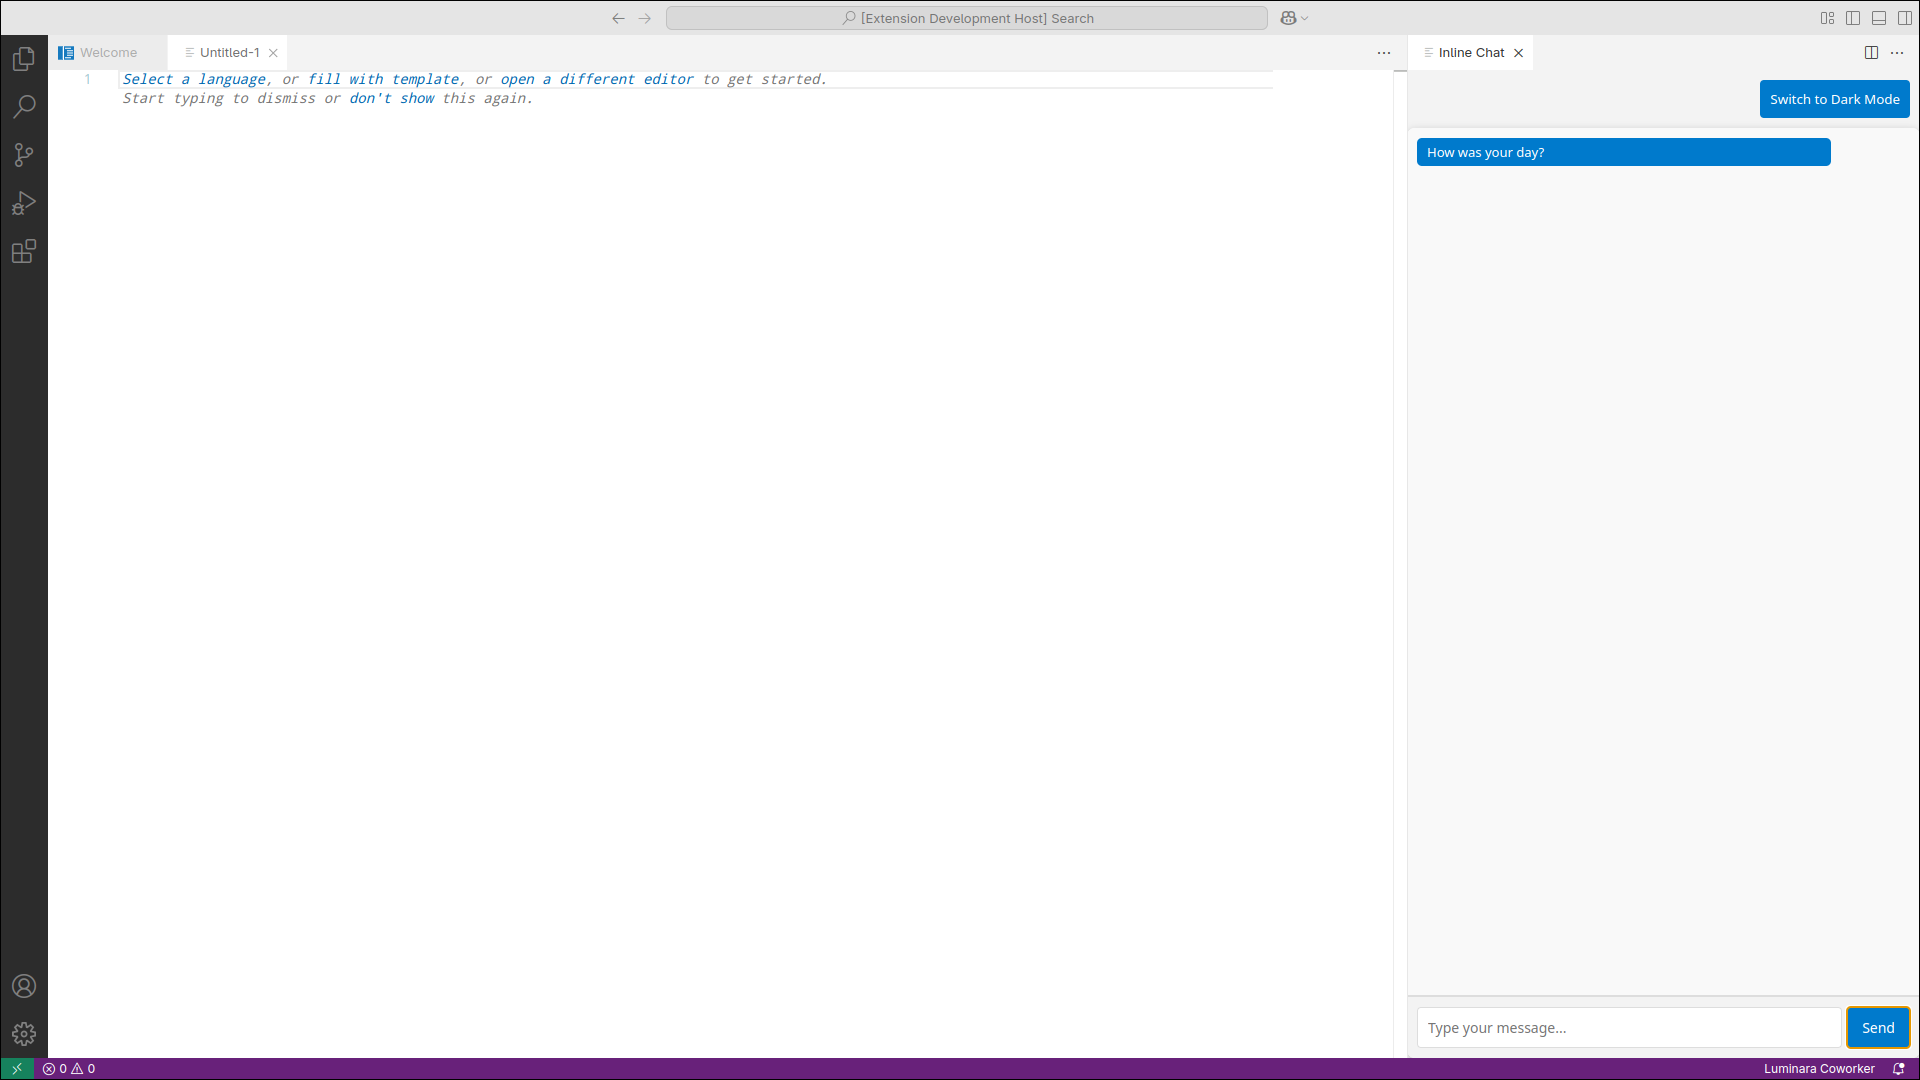
\includegraphics[width=\textwidth]{VSCodeExtension.png}
  \end{columns}
\end{frame}

\begin{frame}{Risks of AI \& Ethical concerns}
  \begin{itemize}
    \item \textbf{Transparency and Data Protection}
    \item \textbf{Bias in training data}
    \item \textbf{Accountability}
    \item \textbf{Job displacement}
  \end{itemize}
\end{frame}

\begin{frame}[plain]
  % Background HTL logo with transparency
  \begin{tikzpicture}[remember picture,overlay]
    \node[opacity=0.2] at (current page.center) 
      {
\includegraphics[width=0.6\paperwidth]{HTL-logo.jpeg}};
  \end{tikzpicture}
  
  \centering
  \vspace{1cm}
  \Huge Thank You for Your Attention!
\end{frame}

\begin{frame}[plain]
  % Background HTL logo with transparency
  \begin{tikzpicture}[remember picture,overlay]
    \node[opacity=0.2] at (current page.center) 
      {
\includegraphics[width=0.6\paperwidth]{HTL-logo.jpeg}};
  \end{tikzpicture}
  \centering
  \vspace{1cm}
  \Huge Backup slides: Graphes
\end{frame}



% Title Slide
\begin{frame}
  \maketitle
\end{frame}

% Slide: Introduction
% Slide: Introduction
\begin{frame}{Introduction}
  \begin{columns}
    \column{0.7\textwidth}
      \begin{itemize}
        \item \textbf{Presenter:} Luna Schätzle 
        \item \textbf{Objective:} Enable student access to open‑source AI tools
        \item \textbf{Focus:} Evaluate and integrate diverse AI models for different usecases
      \end{itemize}
    \column{0.3\textwidth}
      \centering
      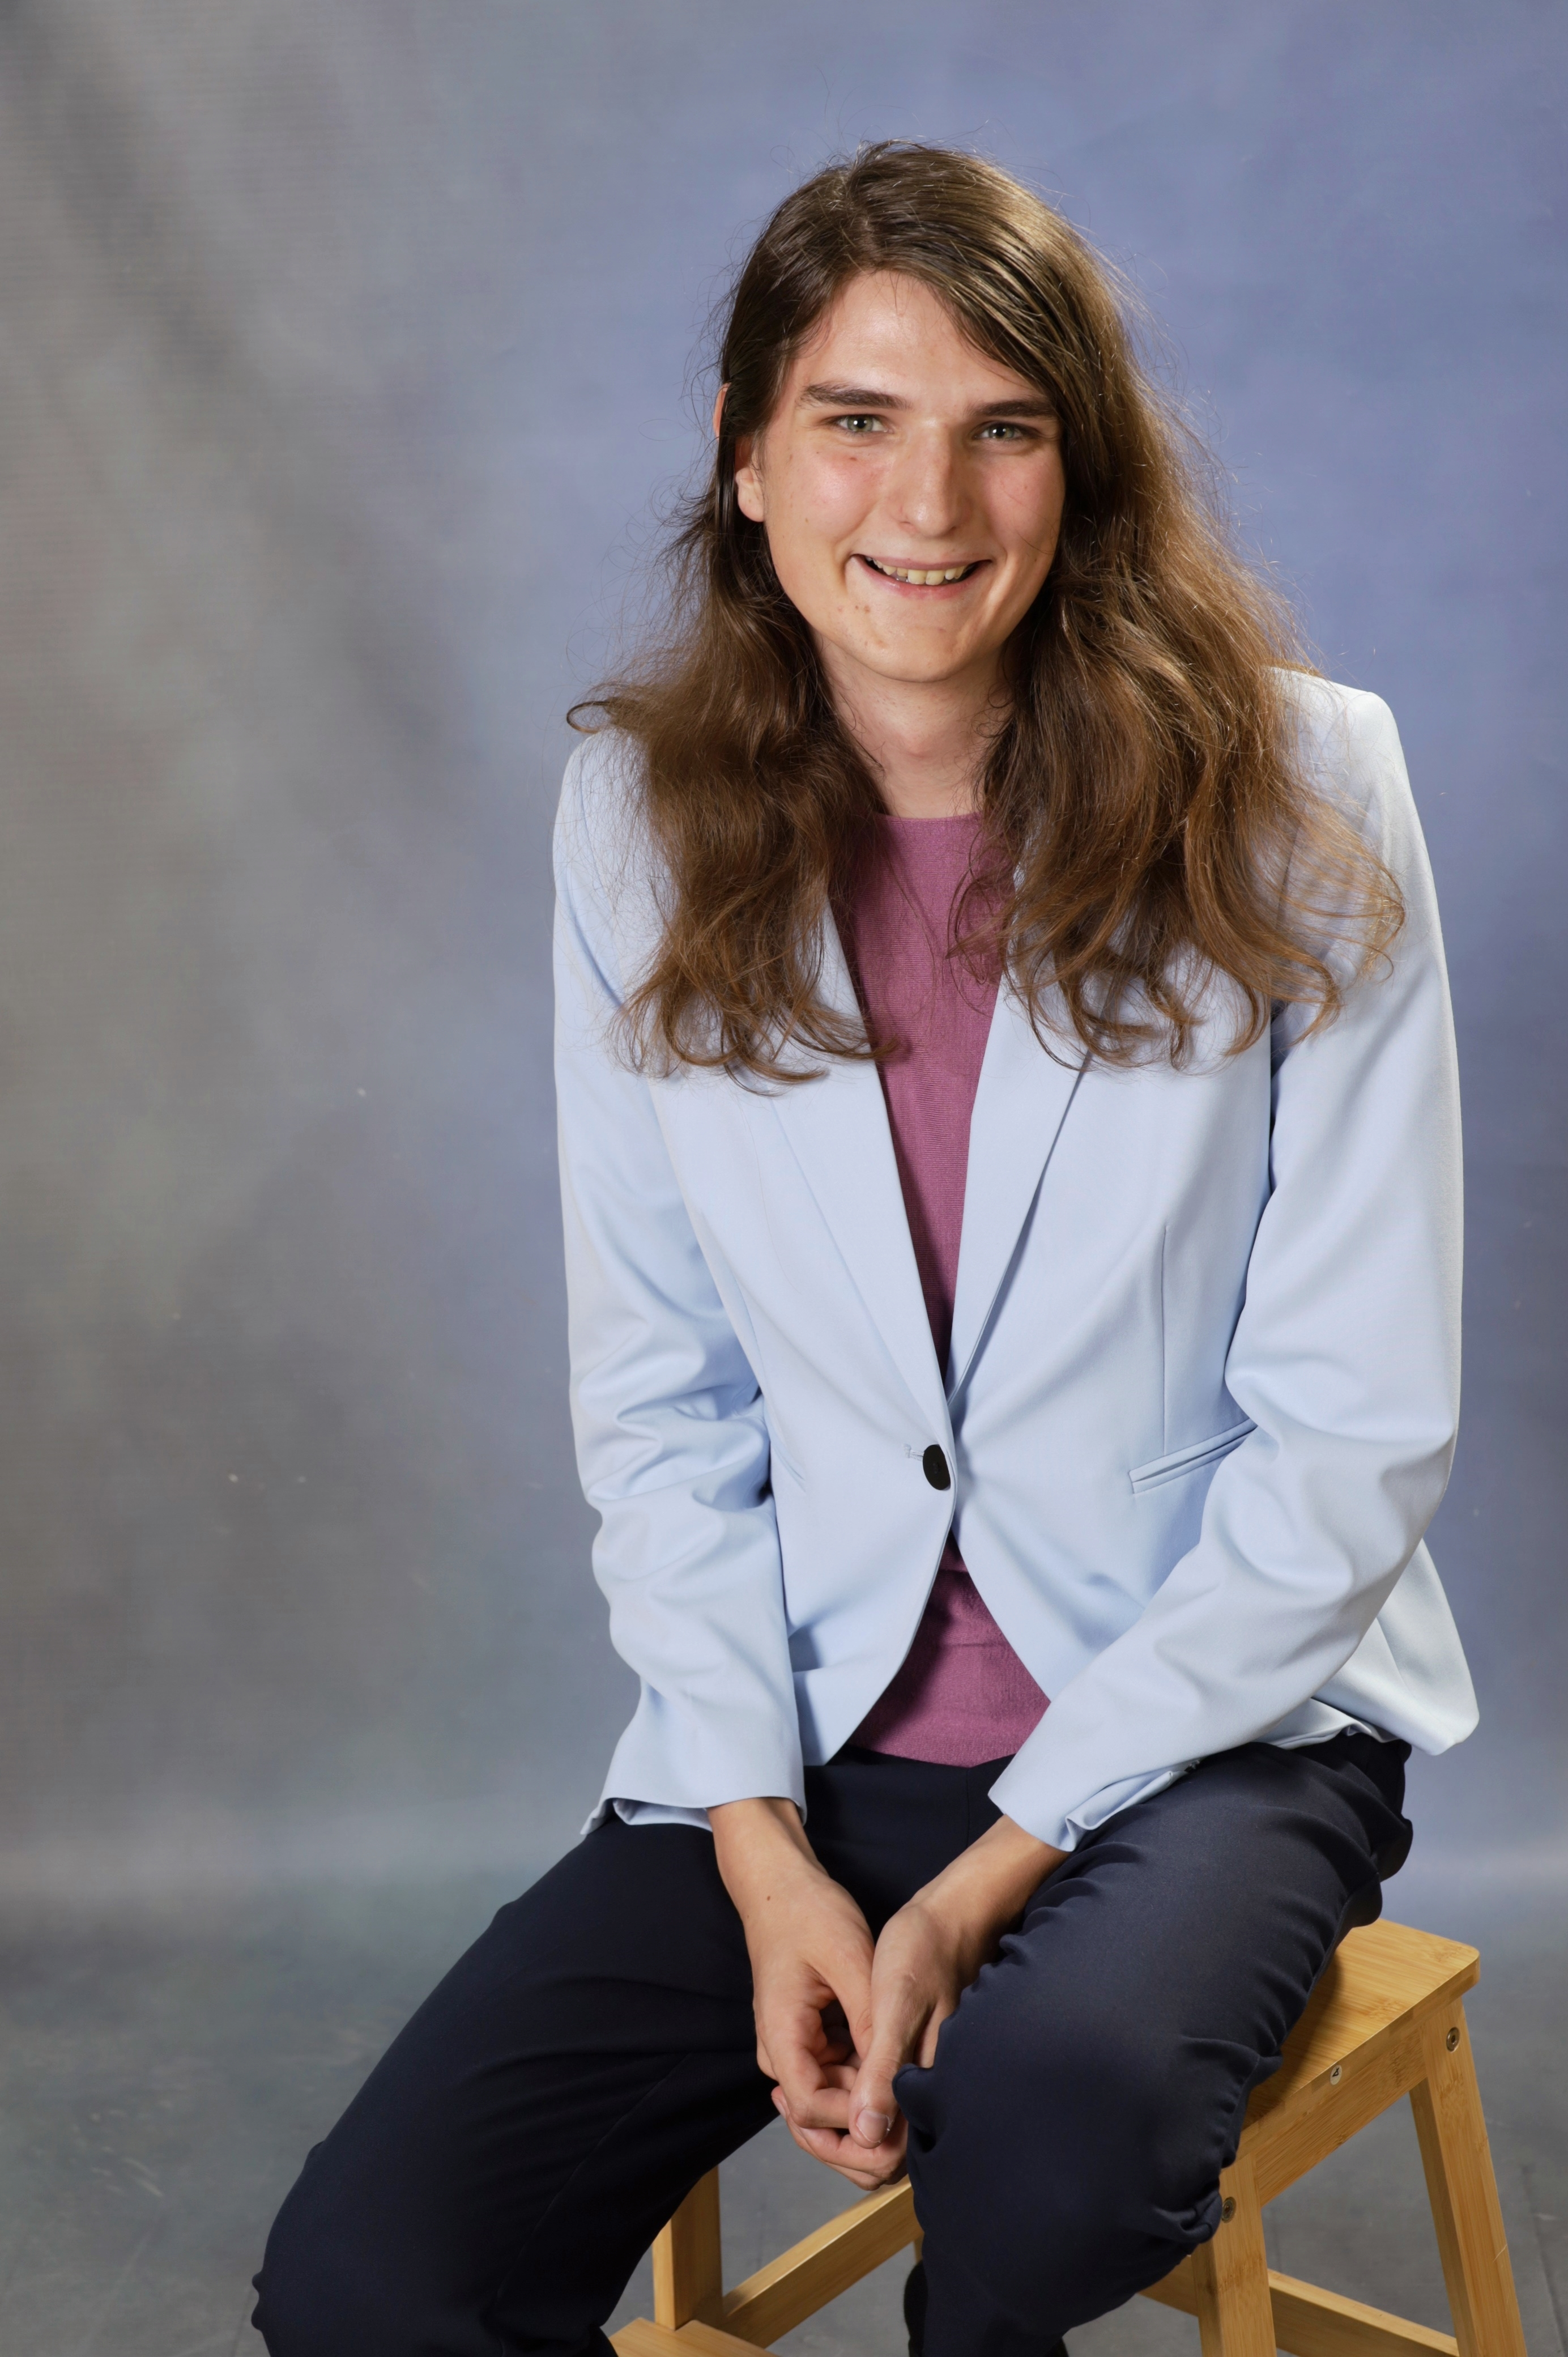
\includegraphics[height=4cm,keepaspectratio]{Luna-Schaetzle.jpg} % Replace with your portrait filename
  \end{columns}
\end{frame}


% Slide: Open Source Impact & Approach
\begin{frame}{Open Source: Impact \& Approach}
  \begin{columns}
    \column{0.80\textwidth}
      \begin{itemize}
        \item \textbf{Definition:} Public, collaborative development
        \item \textbf{Benefits:} Cost-efficient, flexible, and secure via community review
        \item \textbf{Impact:} Fuels innovation and startup growth
        \item \textbf{Approach:} Leverage Python, Flask, and Vue.js
        \item \textbf{Licensing:} Released under GNU GPL-3.0
      \end{itemize}
    \column{0.20\textwidth}
      \centering
      
\includegraphics[width=\textwidth]{Open-Source.png} % Replace with a relevant image
  \end{columns}
\end{frame}


% Slide: Testing and Evaluation
\begin{frame}{Testing and Evaluation}
  \begin{itemize}
    \item \textbf{Models Evaluated:} Llama3.2, Deepseek-r1, Gemma2, Qwen, etc.
    \item \textbf{Methods:} Automated testing with varied prompts via Python scripts.
    \item \textbf{Criteria:}
      \begin{itemize}
        \item Response time
        \item Resource utilization
        \item Accuracy
        \item Readability and text quality
      \end{itemize}
  \end{itemize}
  %\vspace{0.3cm}
  %\centering
  %
\includegraphics[width=0.6\textwidth]{Model-Evaluation.png} % Replace with a representative chart or graphic
\end{frame}

% Slide: Evaluation Results
\begin{frame}{Evaluation Results}
  \begin{itemize}
    \item \textbf{Visualization:} Plots reveal key model discrepancies
    \item \textbf{Performance:} Slight variations in latency, and resource use
    \item \textbf{Efficiency:} Smaller models often outperform larger ones
    \item \textbf{Insight:} Model size alone does not predict quality
    \item \textbf{Integration:} User-driven selection with best‑model recommendation
  \end{itemize}
\end{frame}


% Slide: Website Platform
\begin{frame}{Website: Education Platform}
  \begin{columns}
    \column{0.5\textwidth}
      \begin{itemize}
        \item Serves as a centralized portal for accessing various AI tools.
        \item Technologies: Vue.js (Frontend), Flask (Backend API), and Firebase (Authentication).
      \end{itemize}
    \column{0.5\textwidth}
      \centering
      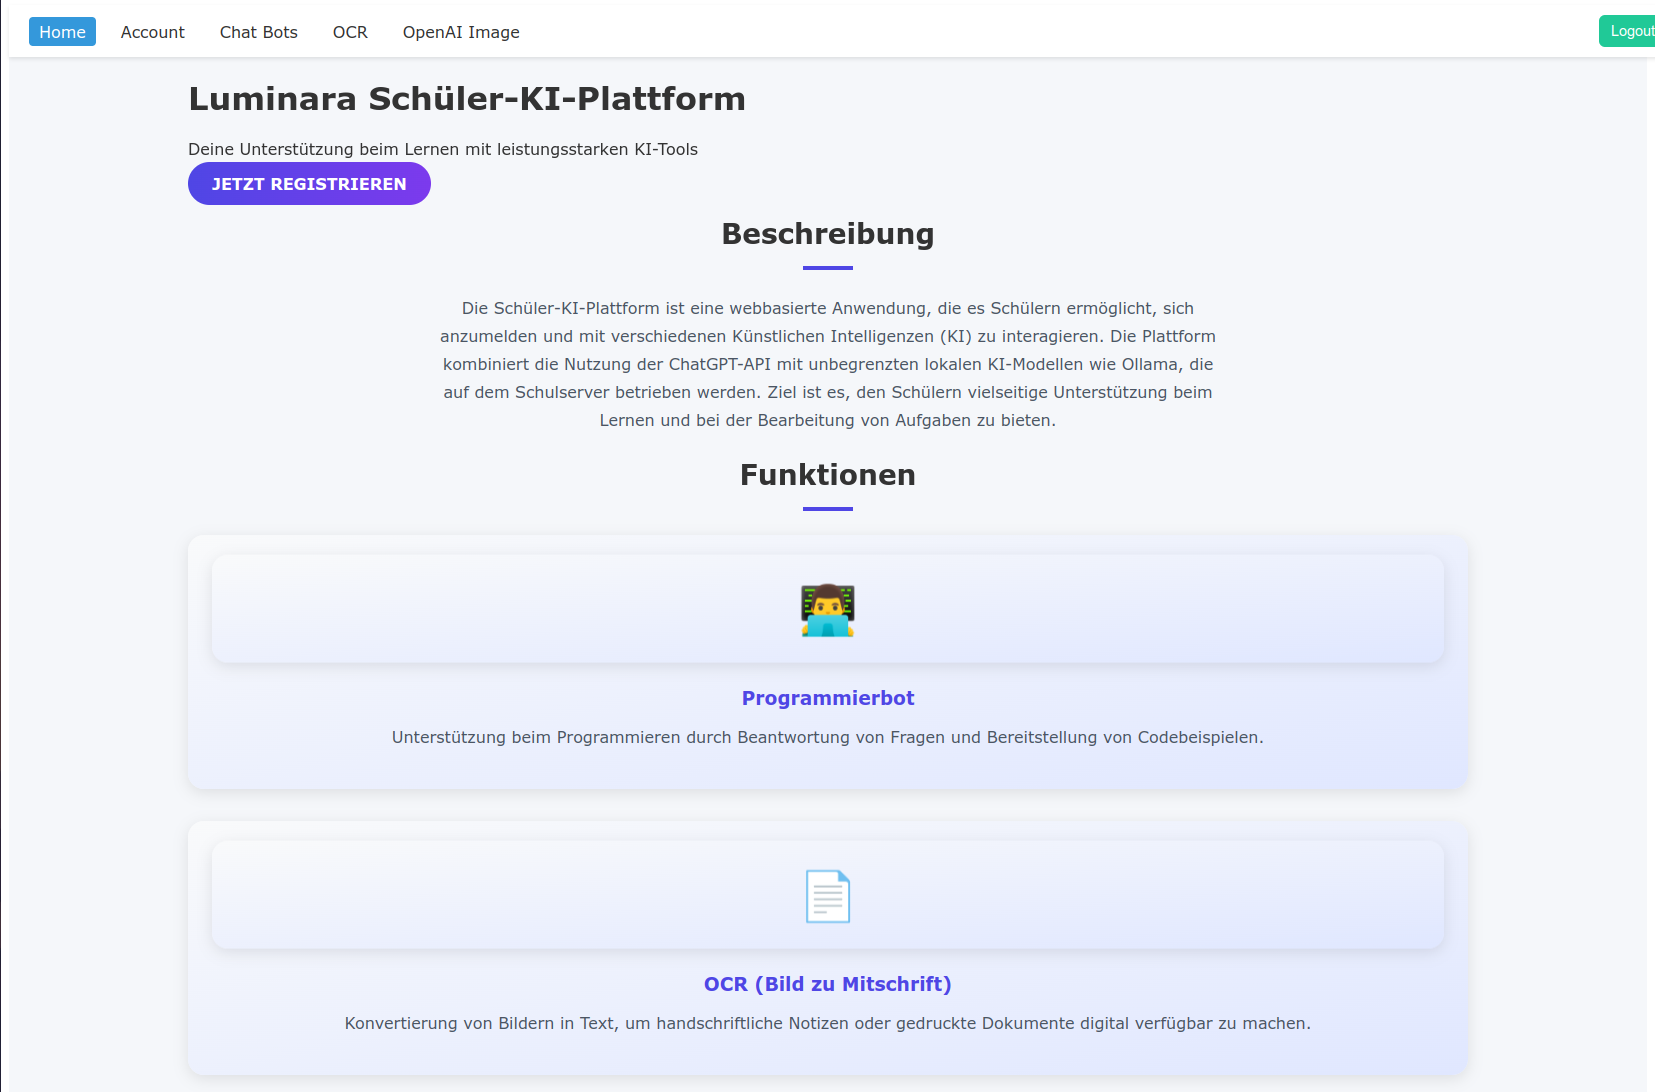
\includegraphics[width=\textwidth]{homepage-screenshot.png}
  \end{columns}
\end{frame}

% Slide: User System
\begin{frame}{User System}
  \begin{columns}
    \column{0.5\textwidth}
      \begin{itemize}
        \item Secure registration and login.
        %\item User profile management.
        \item Firebase-based authentication.
        \item User Dashboard 
      \end{itemize}
    \column{0.5\textwidth}
      \centering
      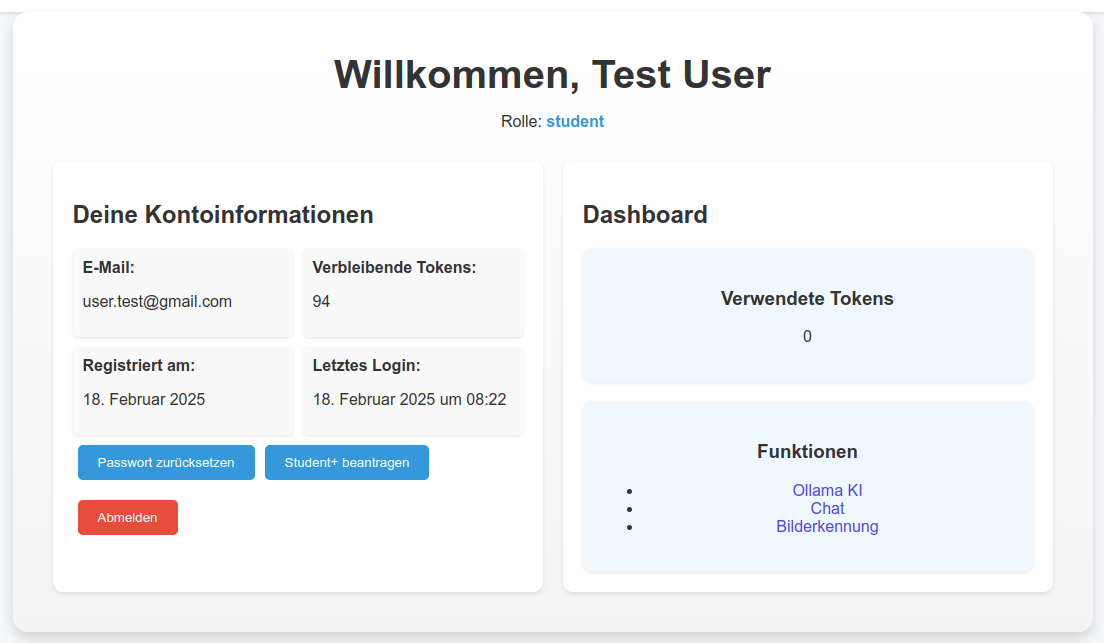
\includegraphics[width=\textwidth]{Account-Managment.png}
  \end{columns}
\end{frame}

% Slide: Chatbot Interface
\begin{frame}{Chatbot Interface}
    \begin{itemize}
        \item Multiple AI models available via a tabbed interface:
            \begin{itemize}
                \item Evaluated models (e.g. Llama3.2, ...)
                \item Vision capabilities: LLaVA, LLaMA 3.2 Vision.
                \item Programming Assistant
                \item ChatGPT (OpenAI API)
            \end{itemize}
    \end{itemize}
    \vspace{0.1cm}
    \centering
    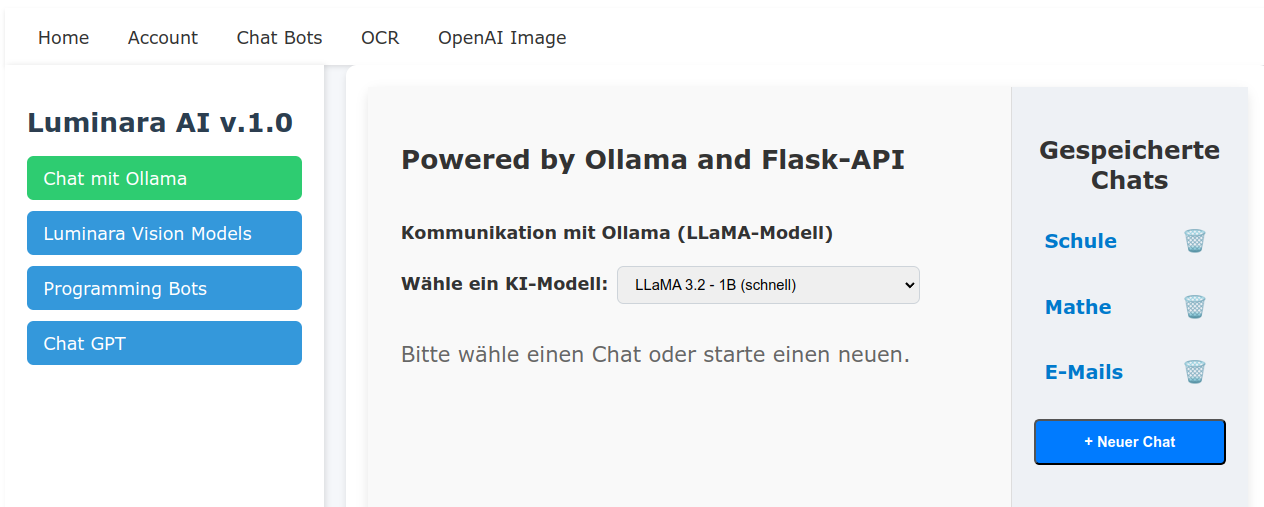
\includegraphics[width=0.65\textwidth]{Chat-Bot-Navigation-Bar.png}
\end{frame}

% Slide: Image Generation
\begin{frame}{Image Generation}
  \begin{columns}
    \column{0.6\textwidth}
      \begin{itemize}
        \item Generate images from text prompts.
        \item Powered by DALL·E (OpenAI).
      \end{itemize}
    \column{0.4\textwidth}
      \centering
      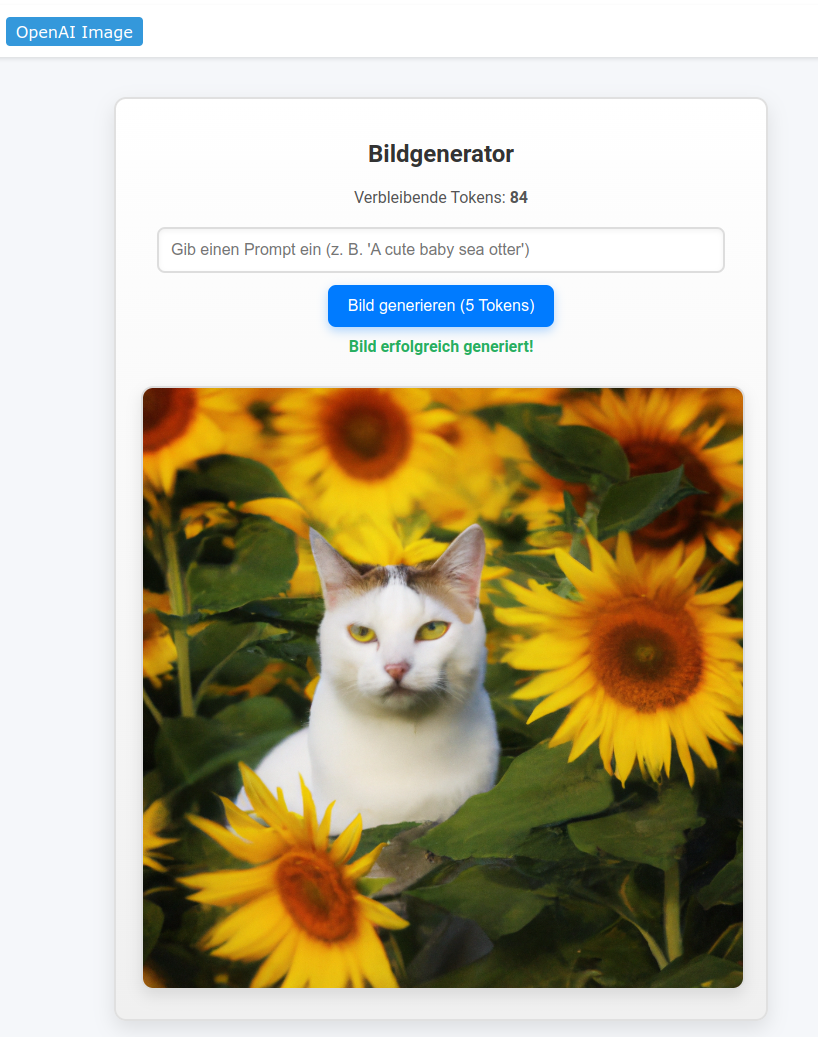
\includegraphics[width=\textwidth]{image-generation.png}
  \end{columns}
\end{frame}

% Slide: OCR and Image Recognition
\begin{frame}{OCR - Obtical Character Recognition}
  \begin{columns}
    \column{0.6\textwidth}
      \begin{itemize}
        \item OCR capabilities using Tesseract.
        \item Post-processing with a large language model.
        \item Outputs formatted using Markdown.
      \end{itemize}
    \column{0.4\textwidth}
      \centering
      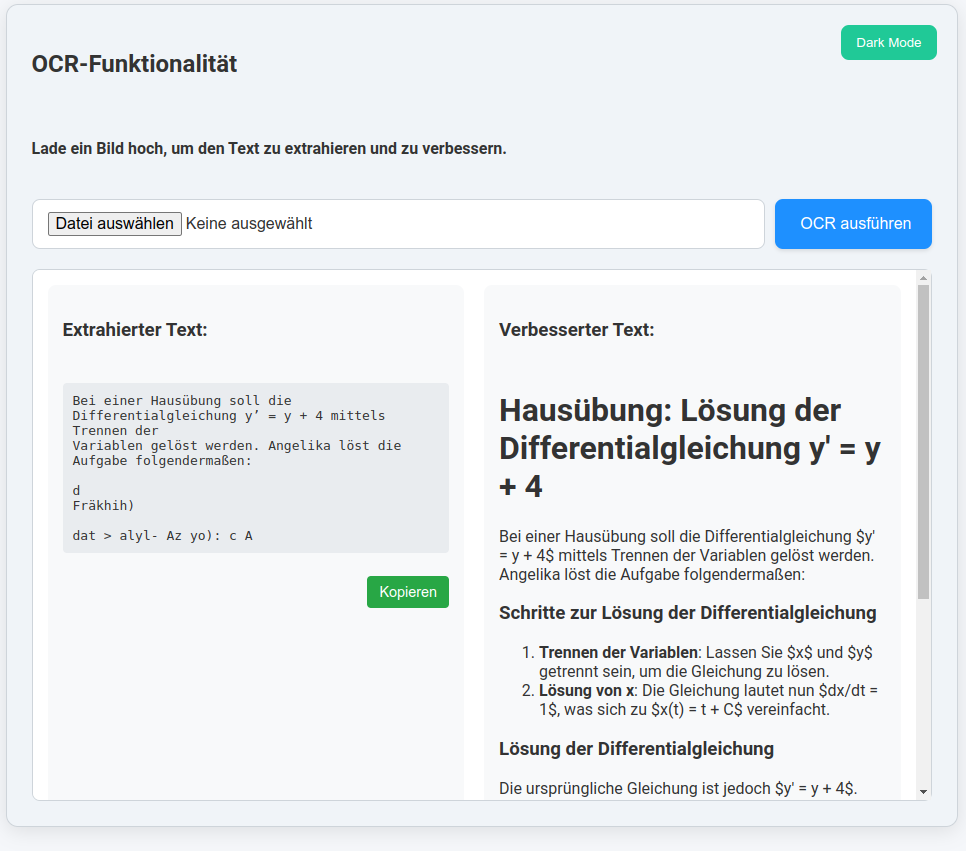
\includegraphics[width=\textwidth]{OCR-functonalatie.png}
  \end{columns}
\end{frame}

% Slide: AI in Economics and Ethics
\begin{frame}{AI in Economics and Ethics}
  \begin{columns}
    \column{0.5\textwidth}
      \textbf{Applications:}
      \begin{itemize}
        \item Customer service \& support
        \item Supply chain management
        \item Predictive \& Data analysis
        \item Process automation
      \end{itemize}
    \column{0.5\textwidth}
    \centering
    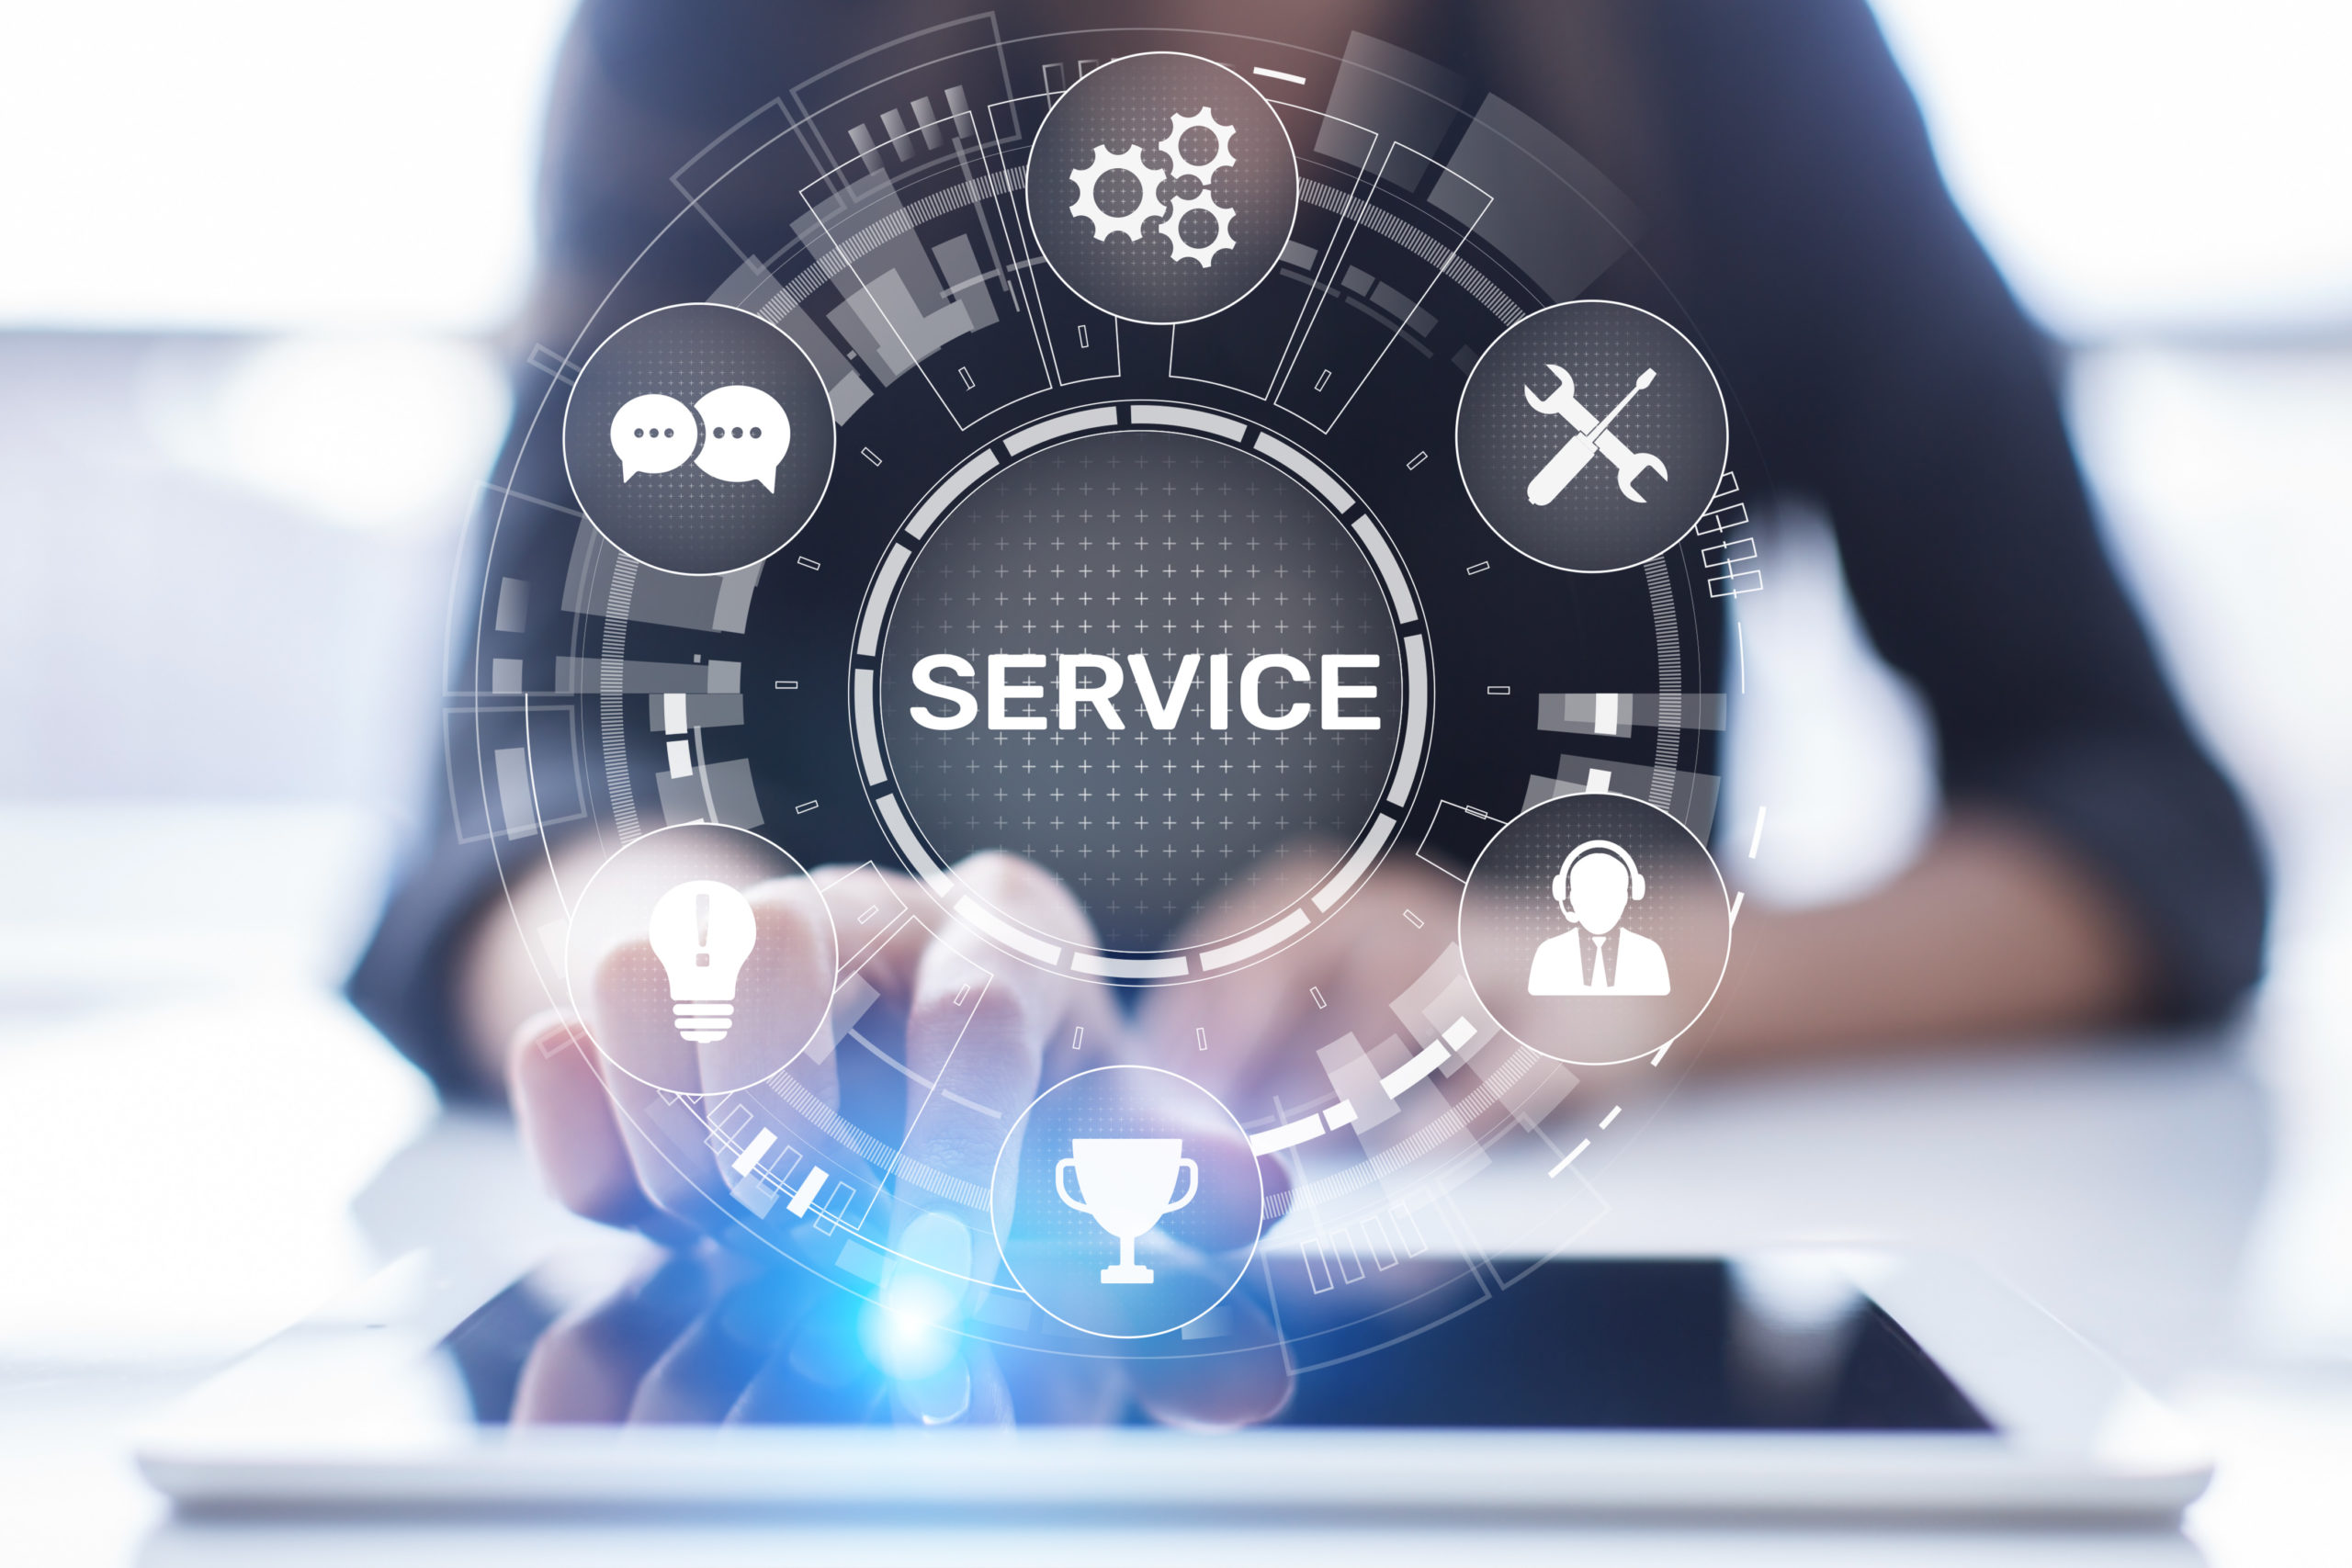
\includegraphics[width=\textwidth]{Customer-Support.png}
  \end{columns}
\end{frame}


% Slide: Regulatory Challenges
\begin{frame}{AI in Economics and Ethics: Regulatory Challenges}
    \begin{columns}
        \column{0.55\textwidth}
            \begin{itemize}
                \item Data security standards \\(GDPR [EUR-Lex: 2016/679])
                \item EU AI Act [EUR-Lex: 2024/1689]
                \item Inconsistent global regulations
            \end{itemize}
        \column{0.45\textwidth}
            \centering
            
\includegraphics[width=\textwidth]{EU-AI-Regulation.png} % Bild hinzufügen, ersetze "regulatory_challenge.png" ggf. mit deinem Bilddateinamen
    \end{columns}
\end{frame}

% Closing Slide
\begin{frame}[plain]
    \centering
    \begin{tikzpicture}[remember picture,overlay]
            \node[opacity=0.1, at=(current page.center)] 
              {
\includegraphics[width=0.5\textwidth]{HTL-logo.jpeg}};
          \end{tikzpicture}
    \Huge Thank You for Your Attention!
\end{frame}


\begin{frame}[plain]
  % Background HTL logo with transparency
  \begin{tikzpicture}[remember picture,overlay]
    \node[opacity=0.2] at (current page.center) 
      {
\includegraphics[width=0.6\paperwidth]{HTL-logo.jpeg}};
  \end{tikzpicture}
  
  \centering
  \vspace{1cm}
  \Huge Backup slides: Graphes
\end{frame}

%backup Slides for possible Questions
%Maby extra slide with the results
\begin{frame}{Evaluation Results: Qualitative metrics}
  \begin{figure}
    \centering
    \begin{minipage}{0.45\textwidth}
      \centering
      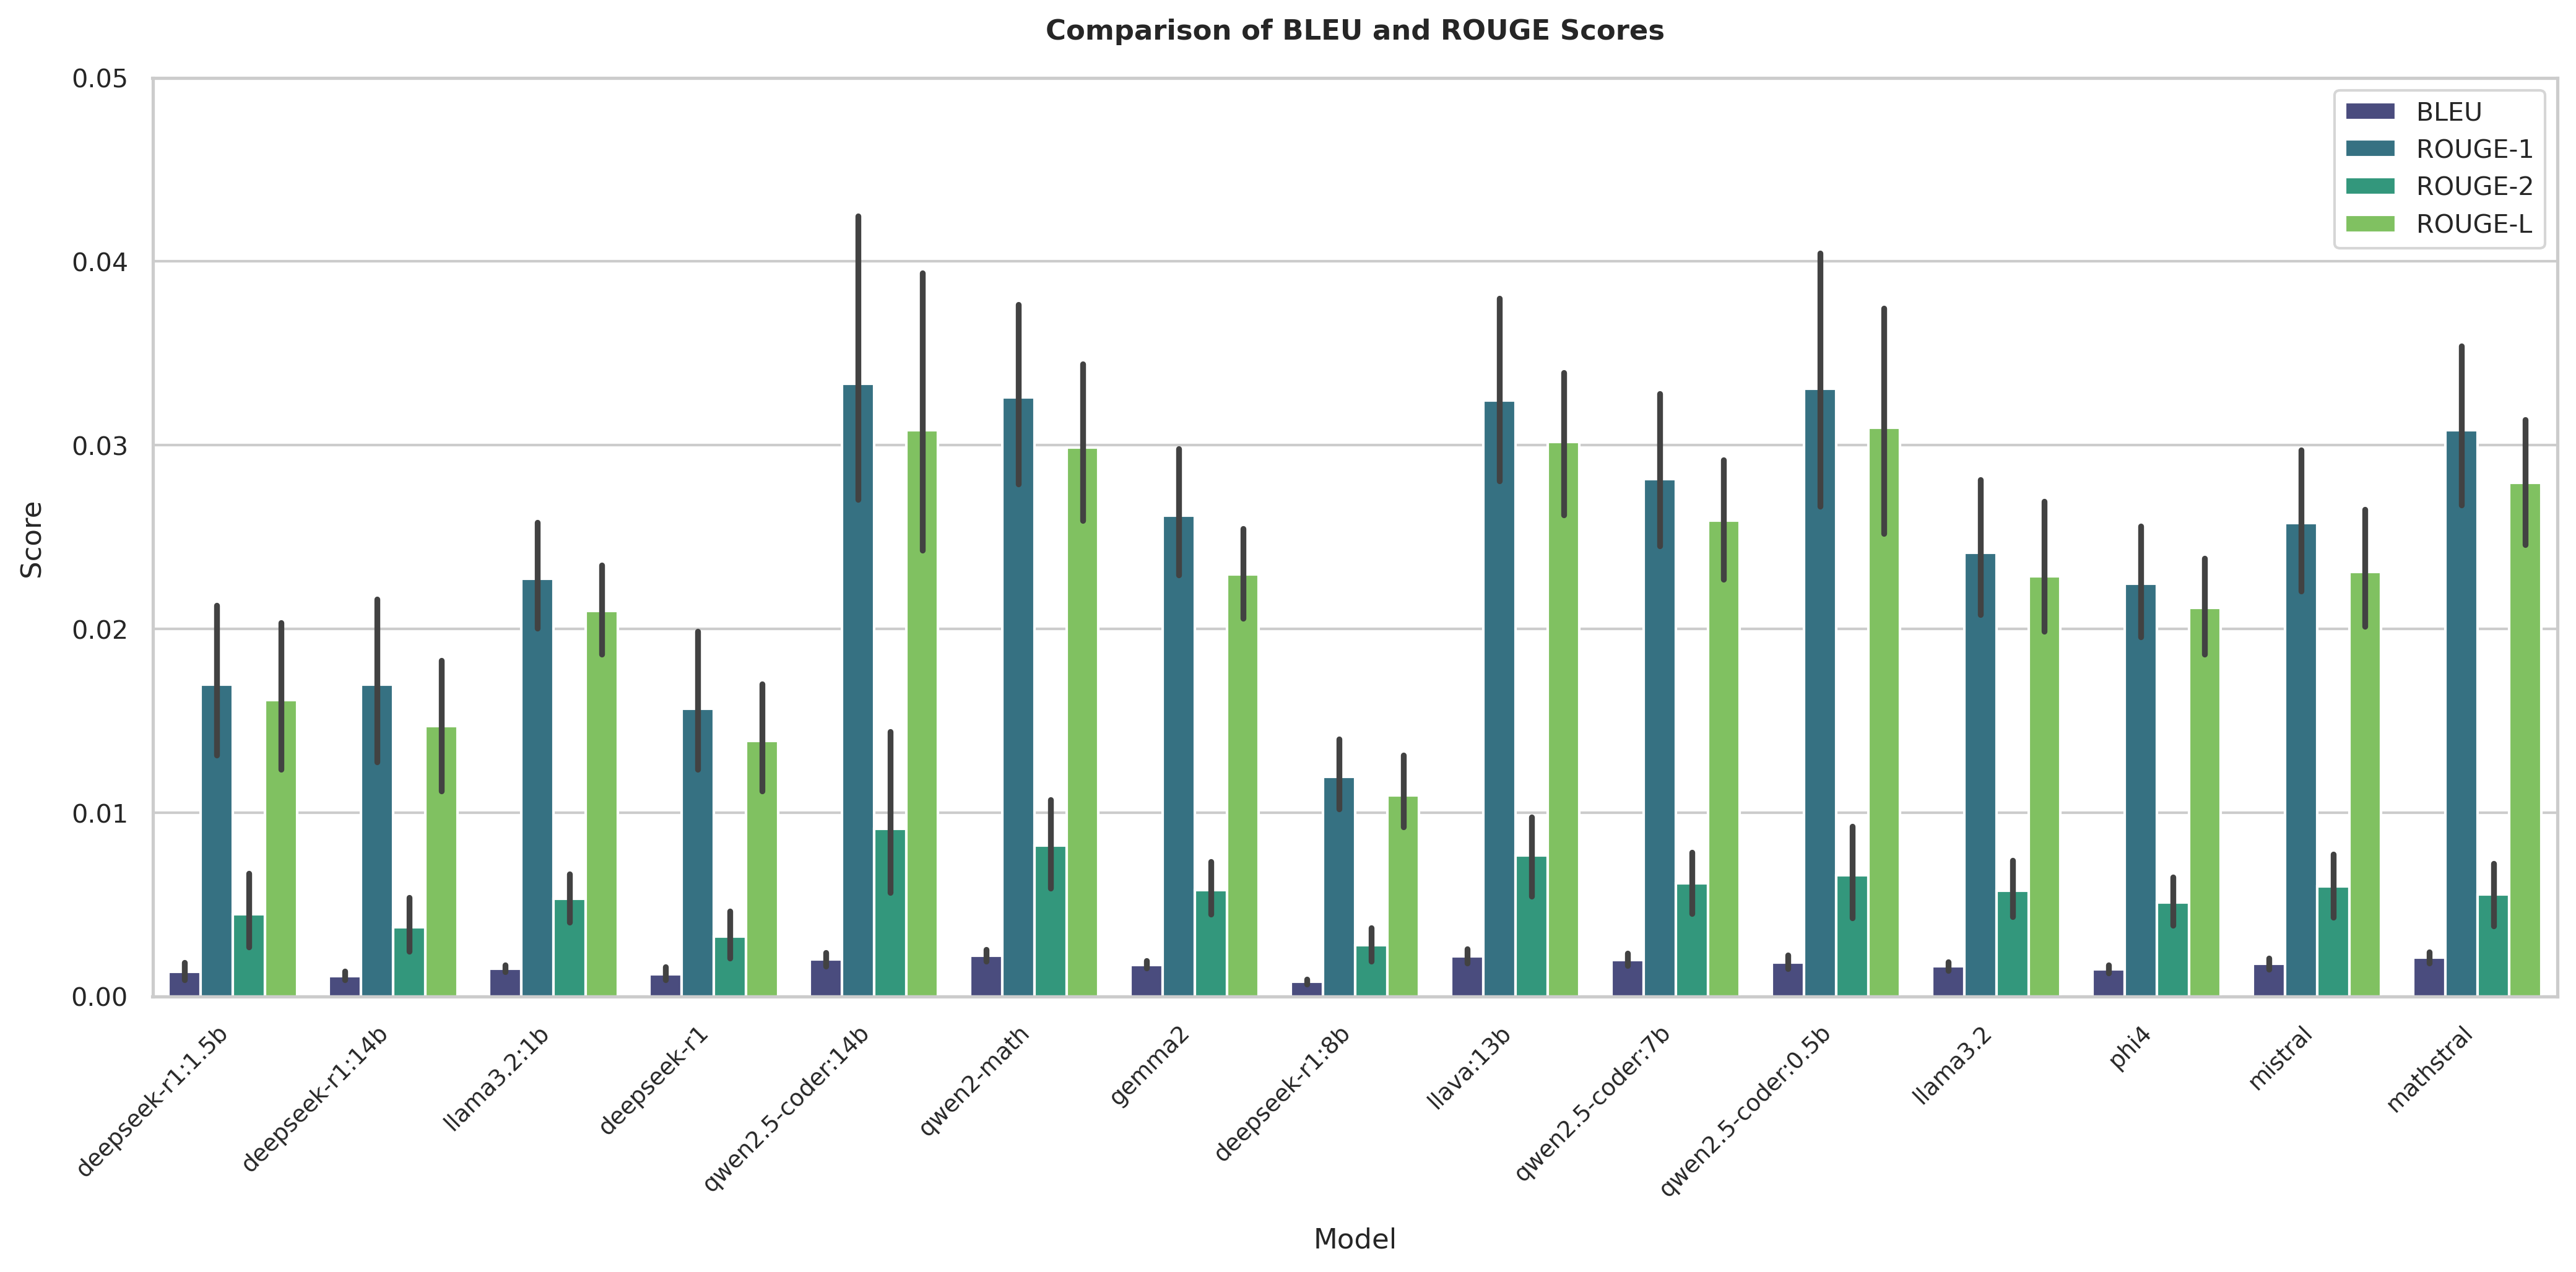
\includegraphics[width=\textwidth]{bleu_rouge.png}
    \end{minipage}
    \hfill
    \begin{minipage}{0.45\textwidth}
      \centering
      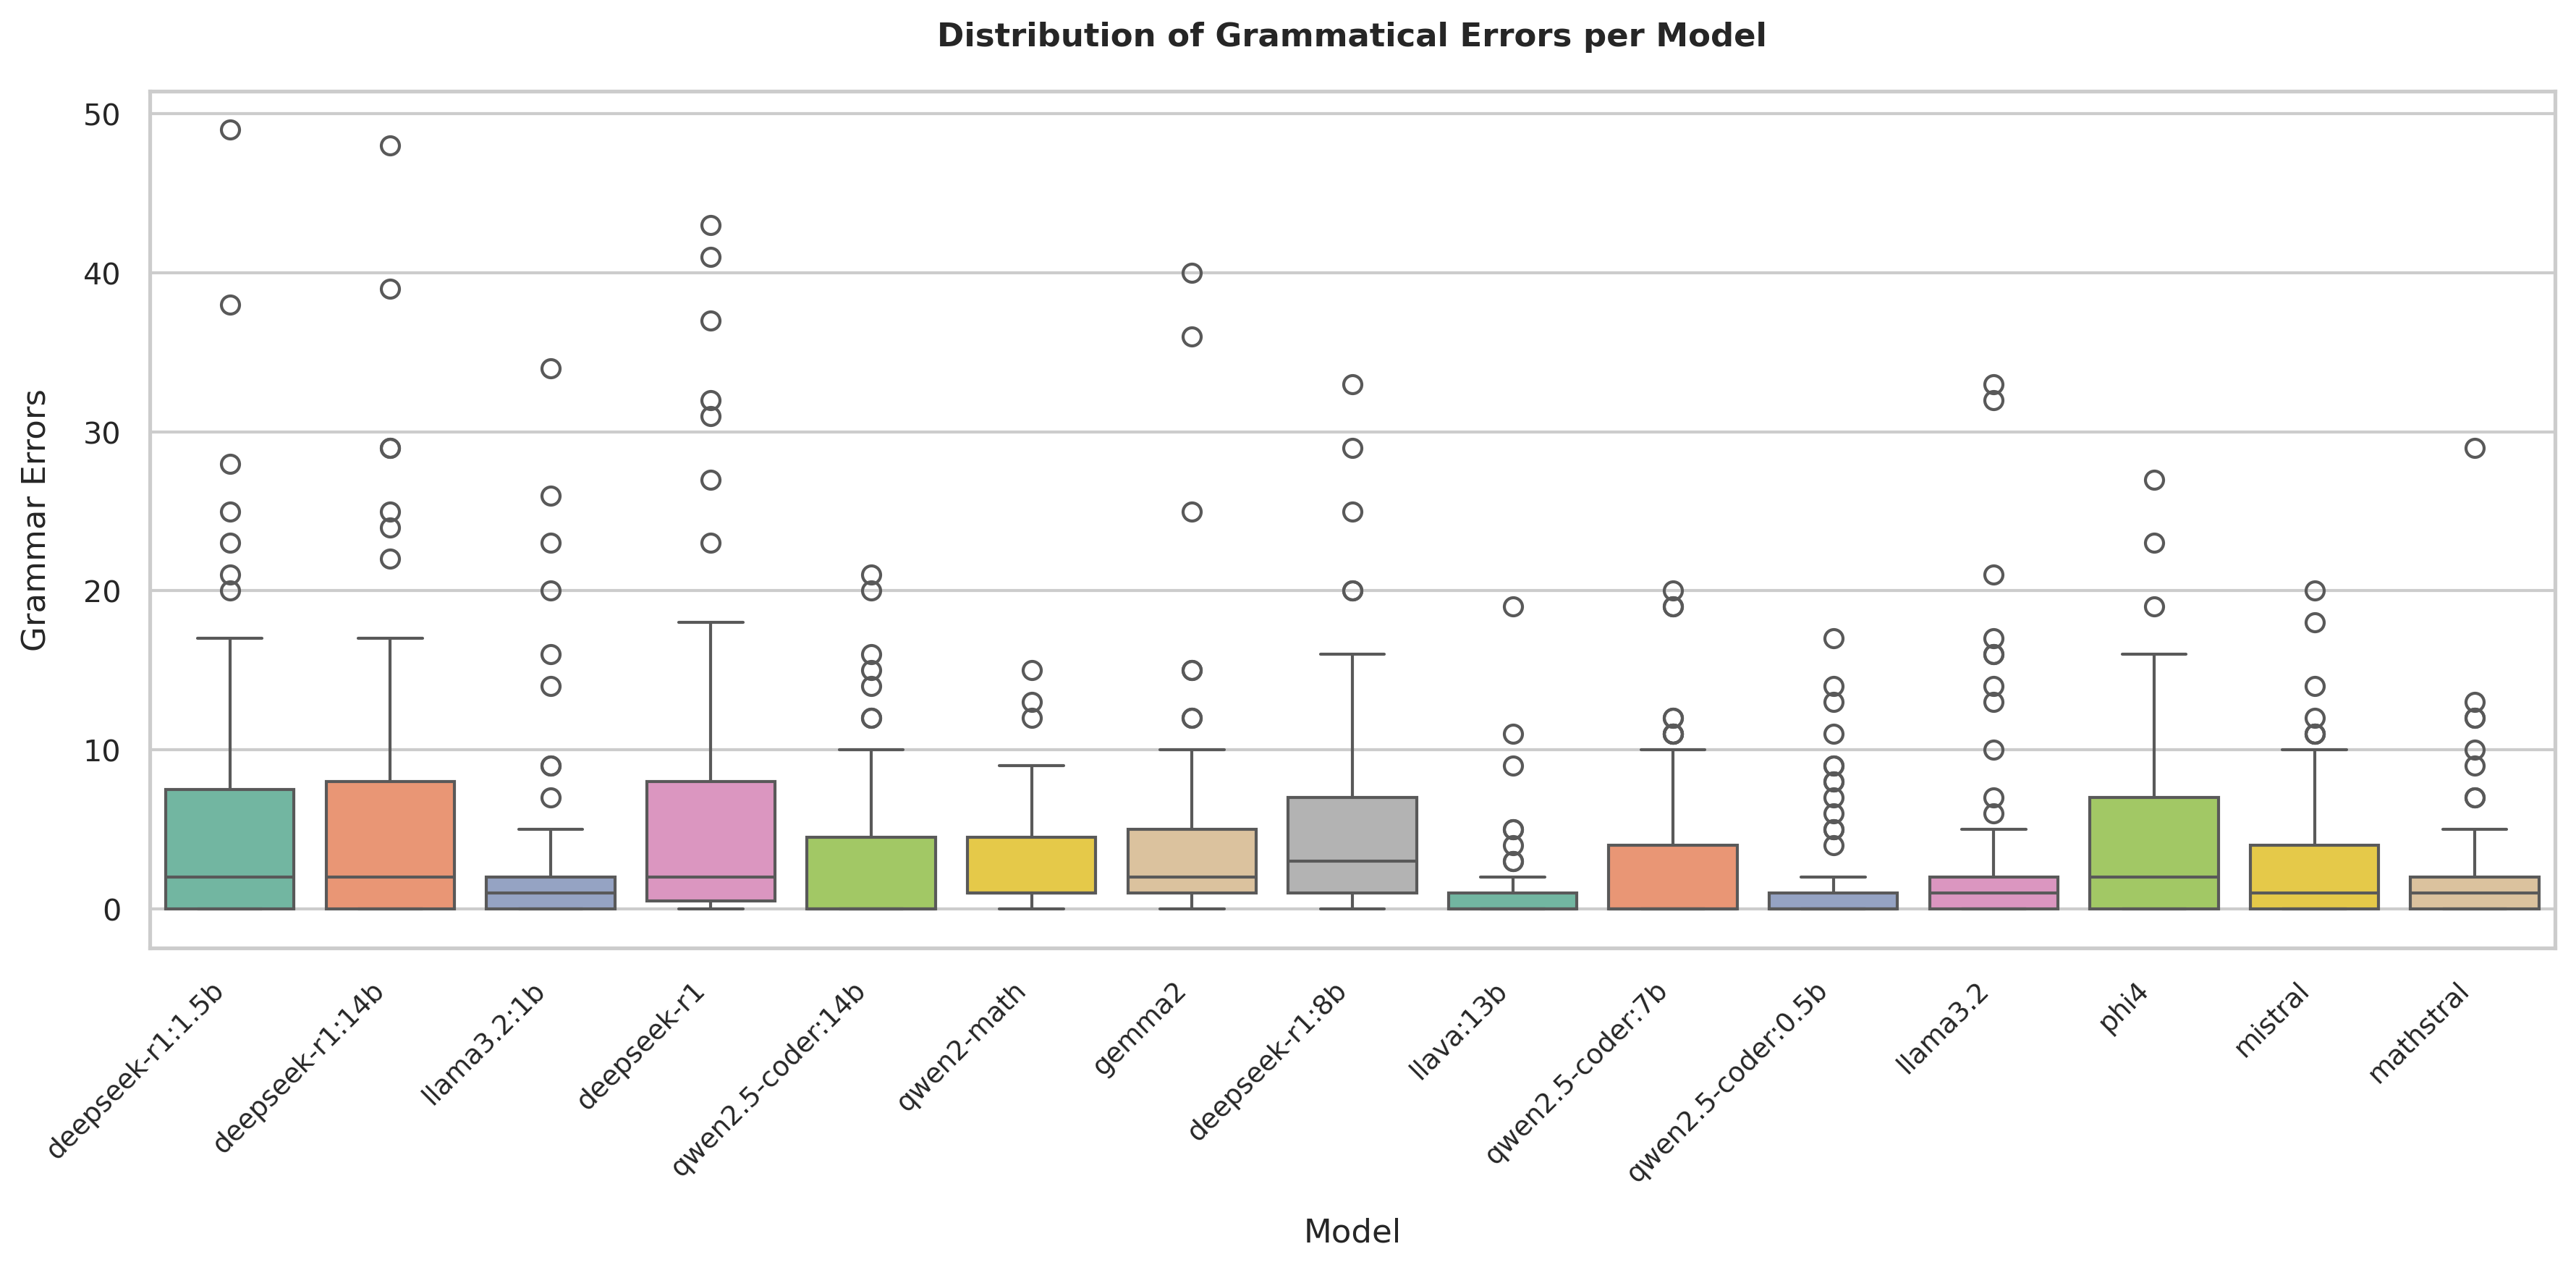
\includegraphics[width=\textwidth]{grammar_errors.png}
    \end{minipage}
    
    \vspace{0.15cm}
    
    \begin{minipage}{0.45\textwidth}
      \centering
      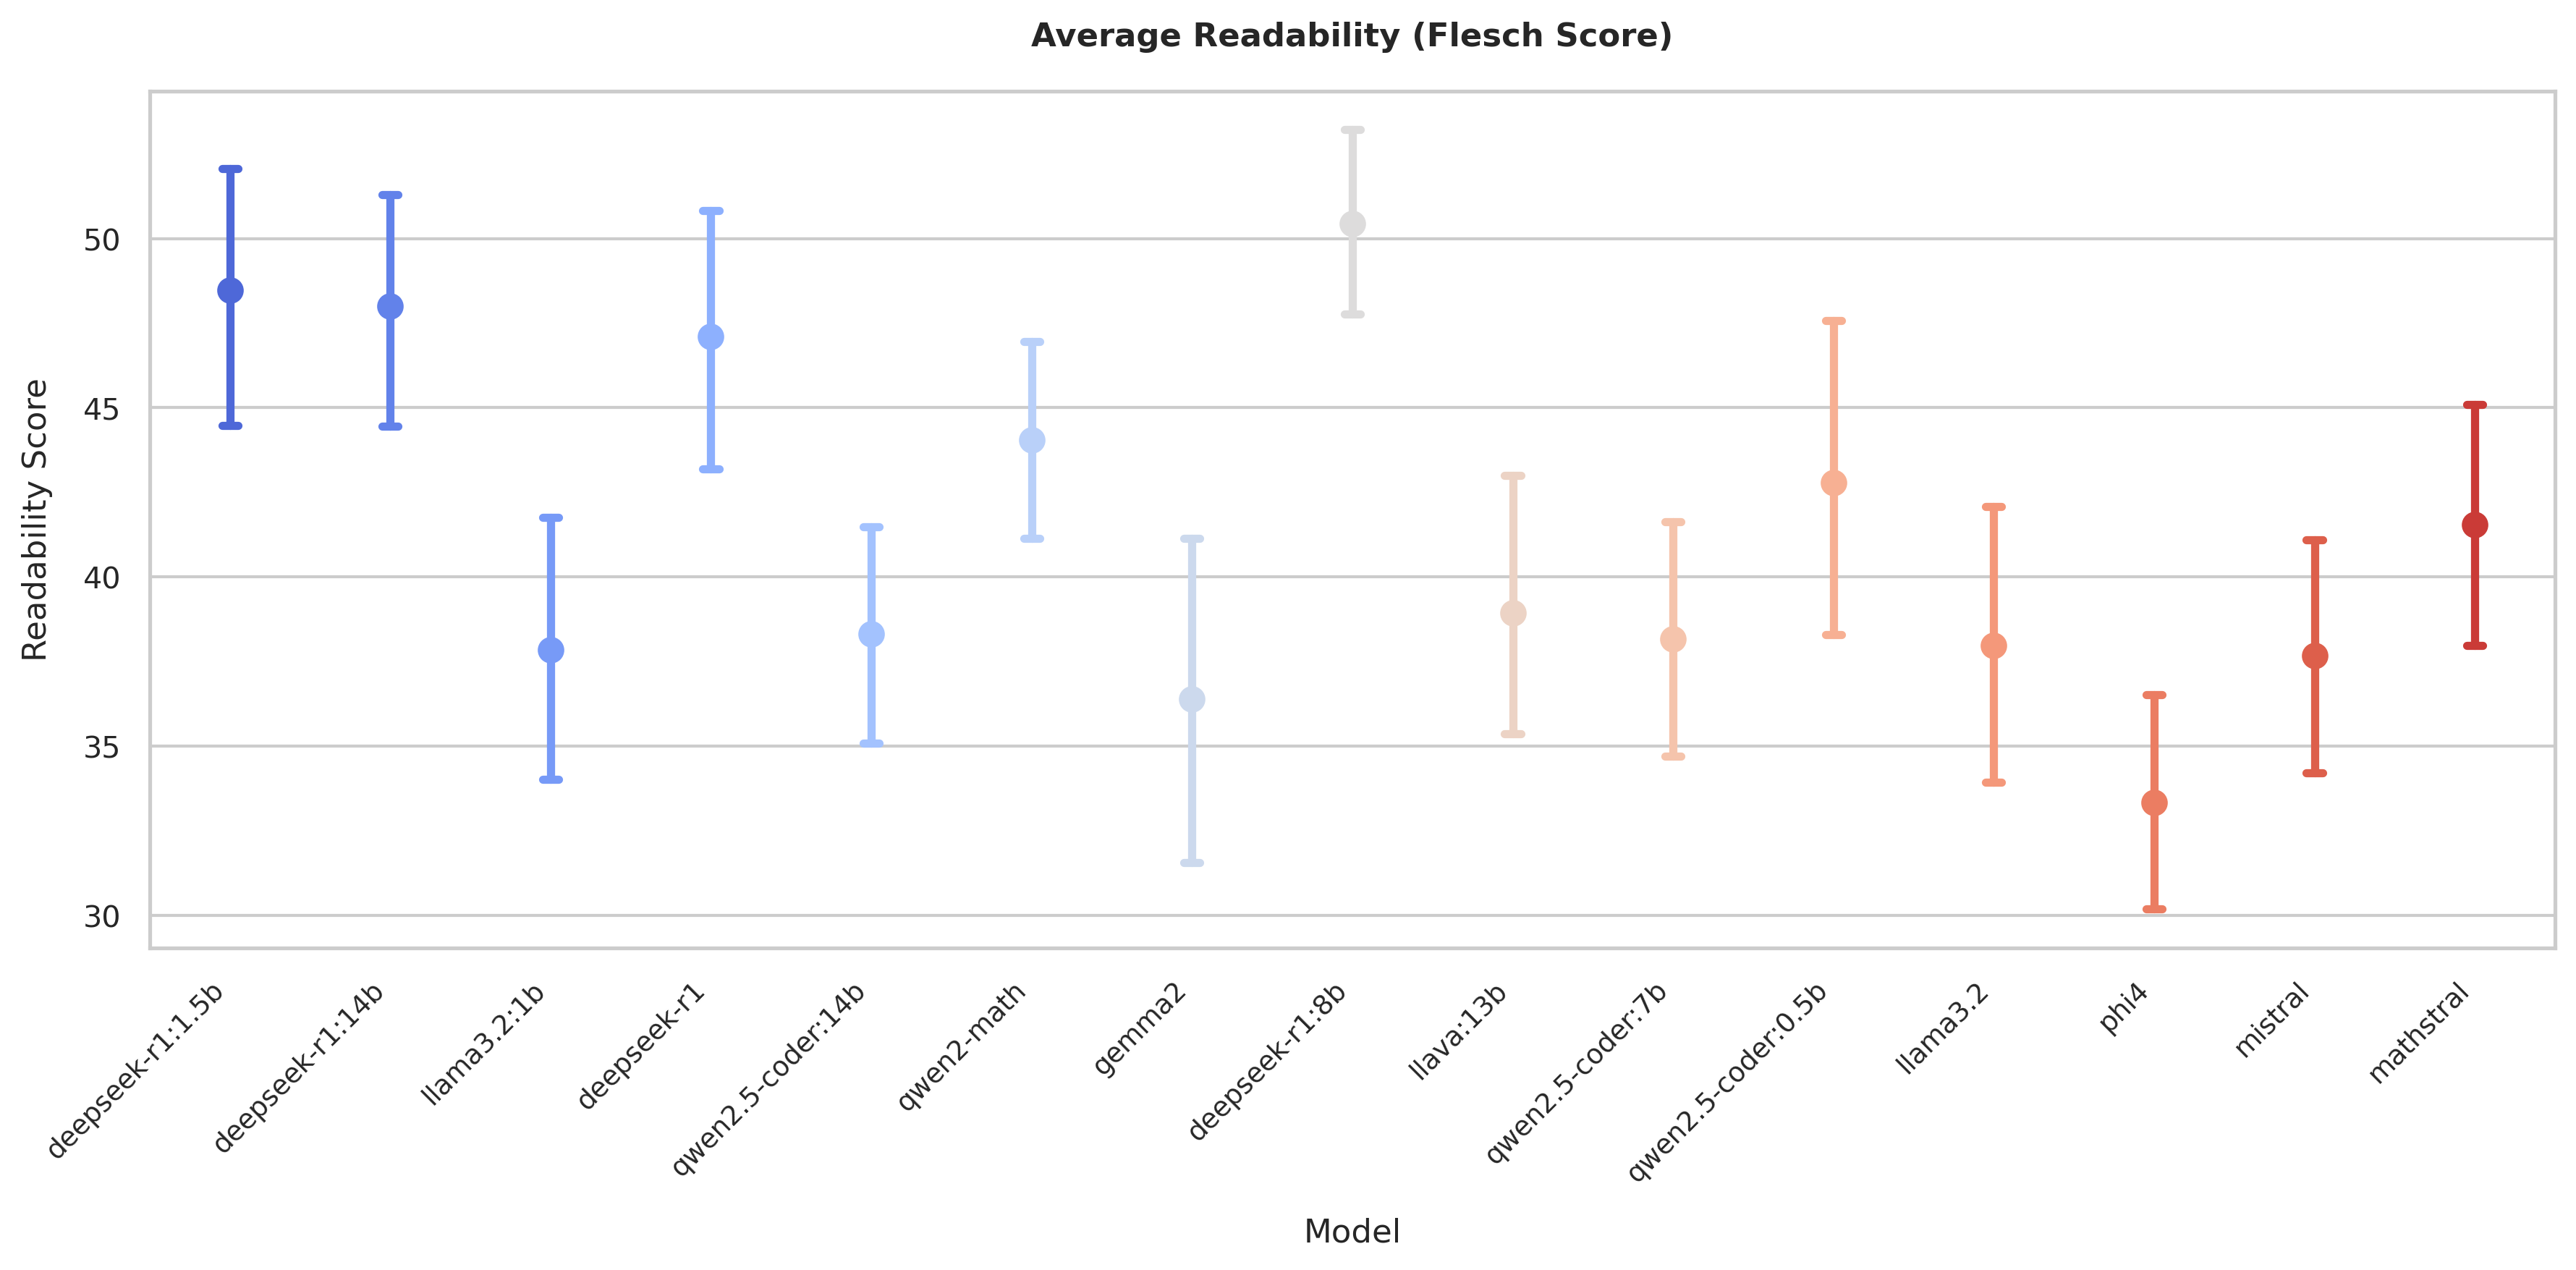
\includegraphics[width=\textwidth]{readability.png}
    \end{minipage}
    \hfill
    \begin{minipage}{0.45\textwidth}
      \centering
      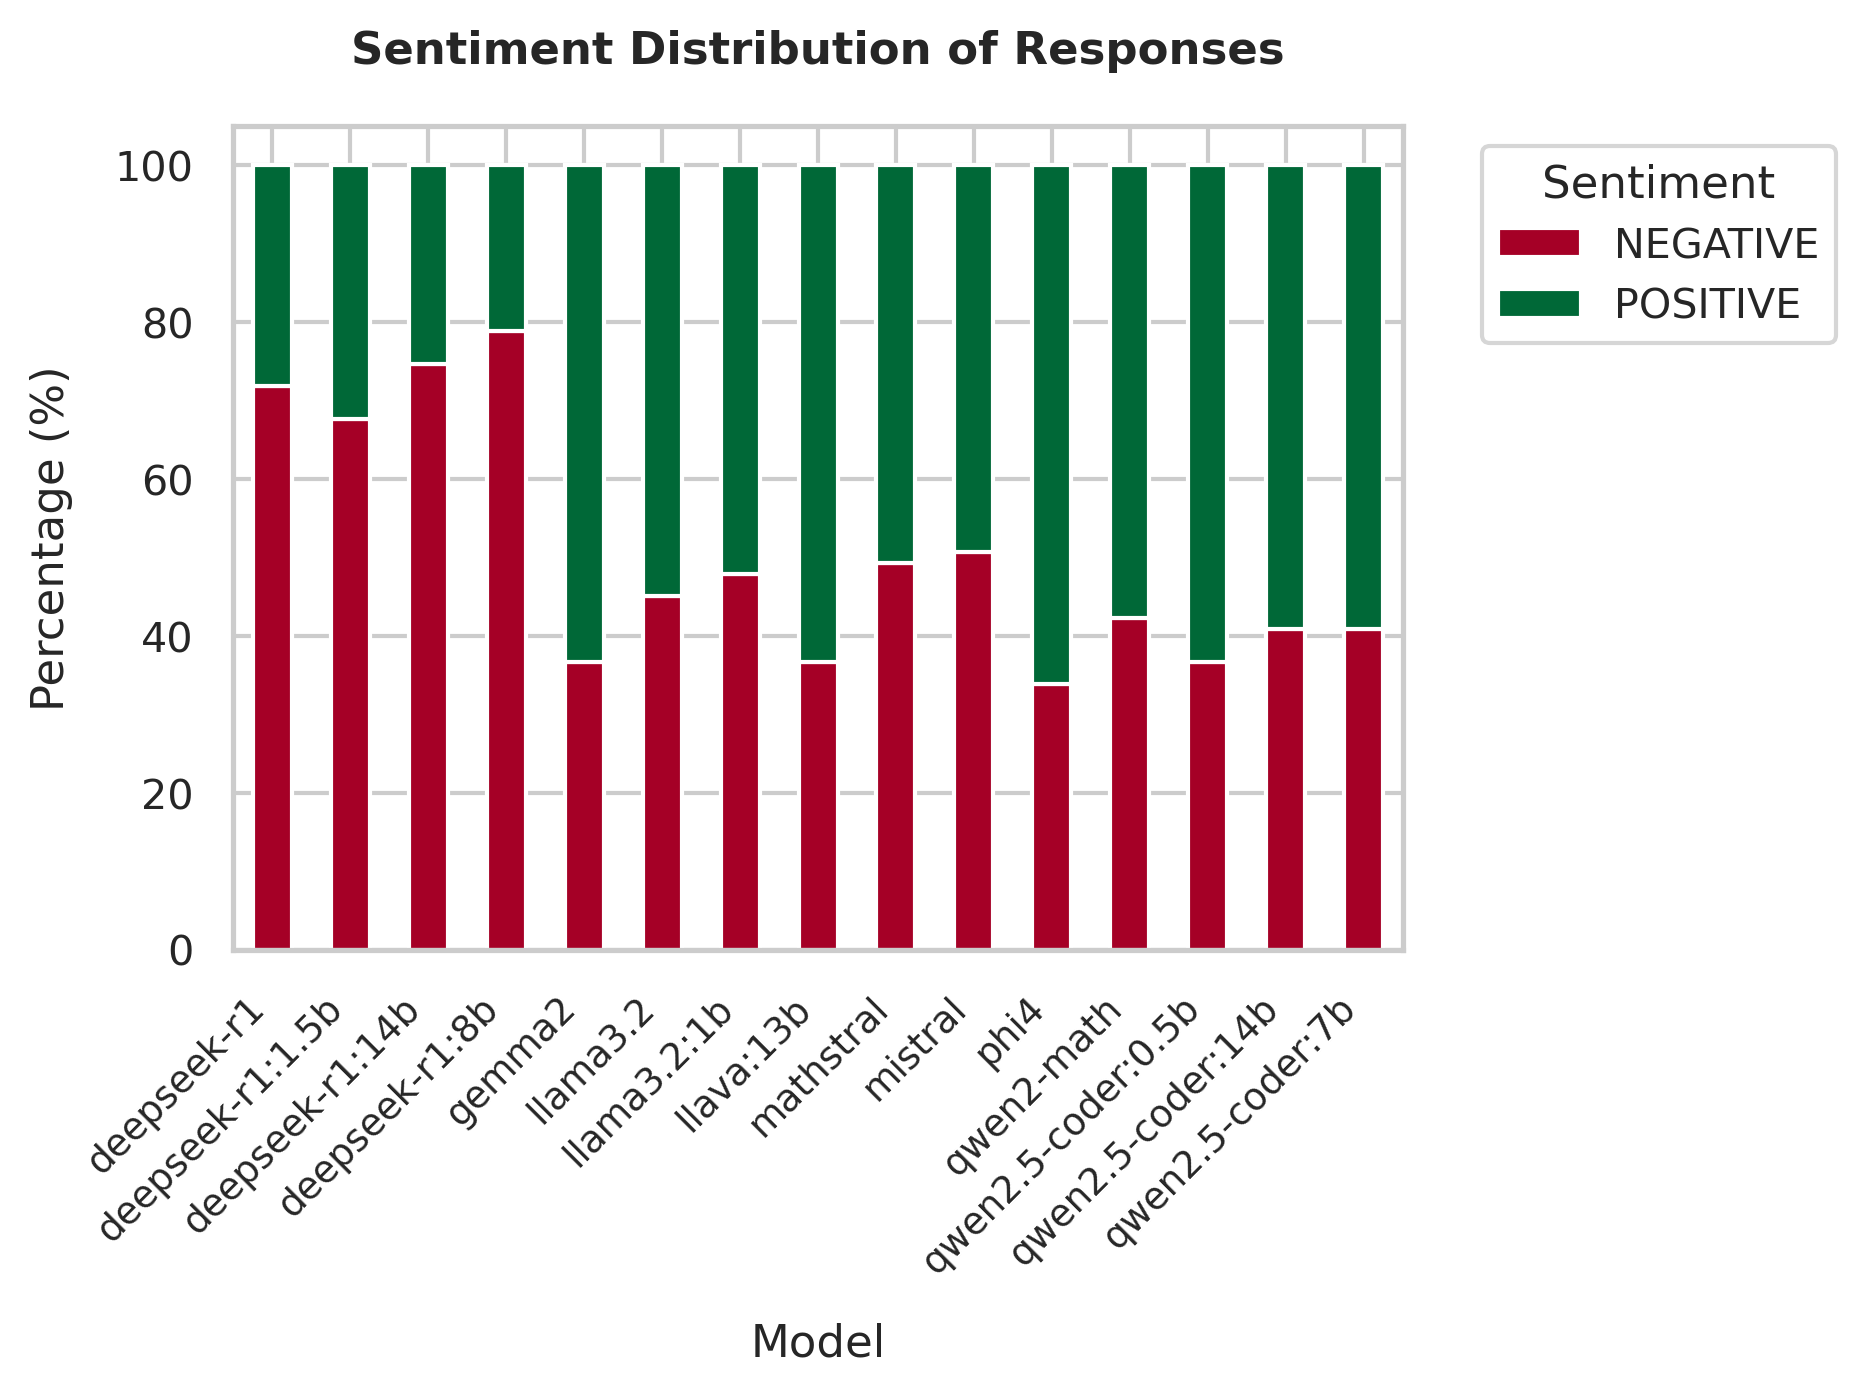
\includegraphics[width=\textwidth]{sentiment.png}
    \end{minipage}
    
    \caption{Evaluation Results of AI Models}
    \label{fig:evaluation-results}
  \end{figure}
\end{frame}

\begin{frame}{Evaluation Results: Quantitative metrics}
  \begin{columns}[t]
    \column{0.5\textwidth}
      \begin{figure}
        \centering
        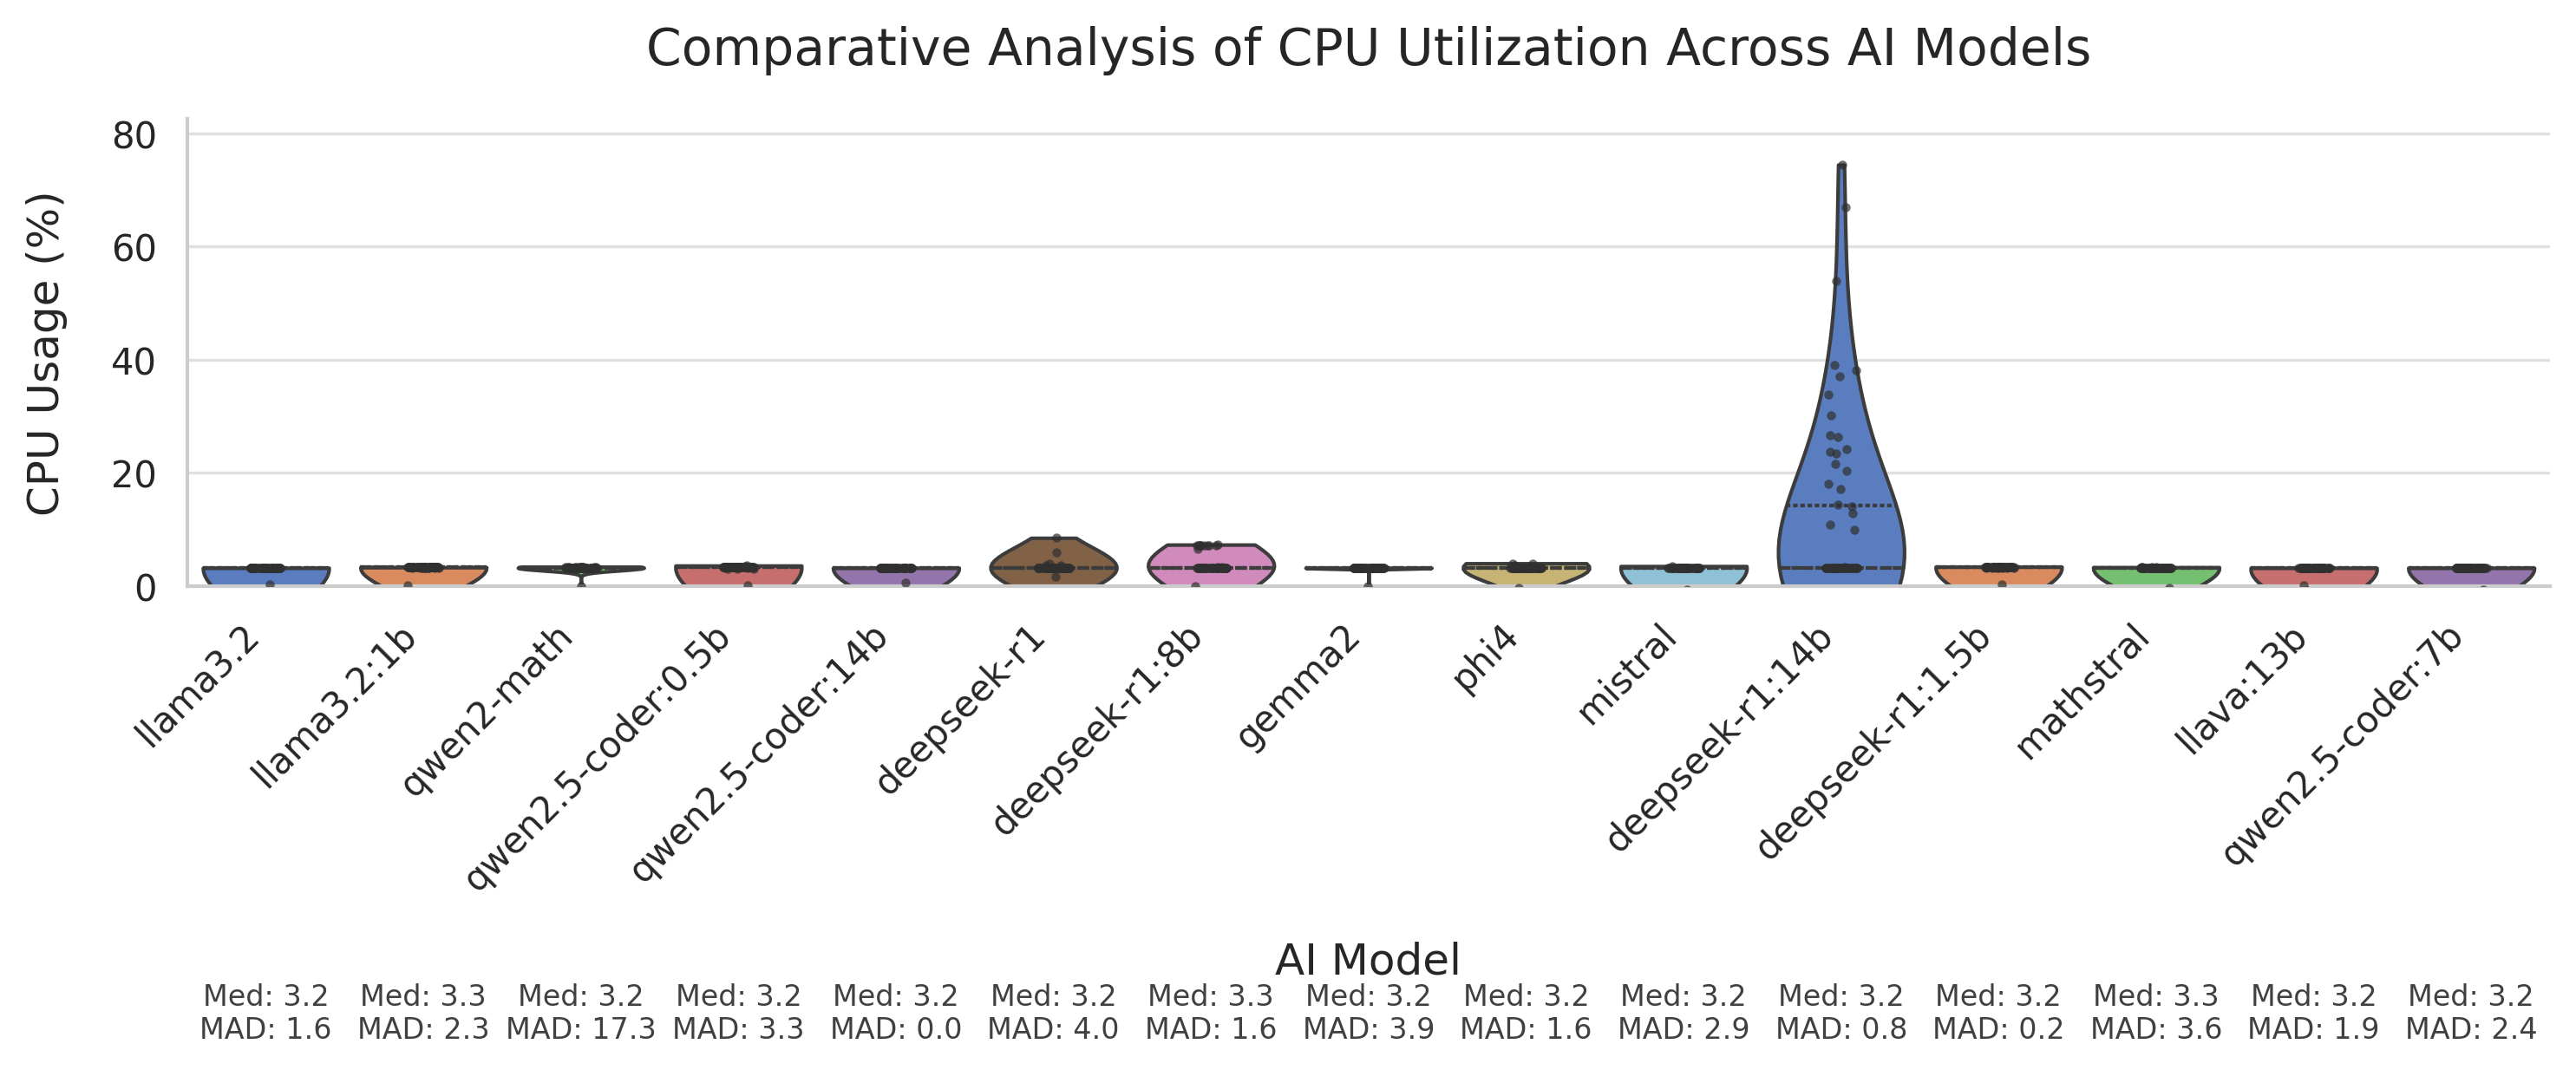
\includegraphics[width=0.9\columnwidth]{model_cpu_usage_comparison.png}
        \caption{CPU Usage Comparison}
        \label{fig:cpu-usage}
      \end{figure}
    \column{0.5\textwidth}
      \begin{figure}
        \centering
        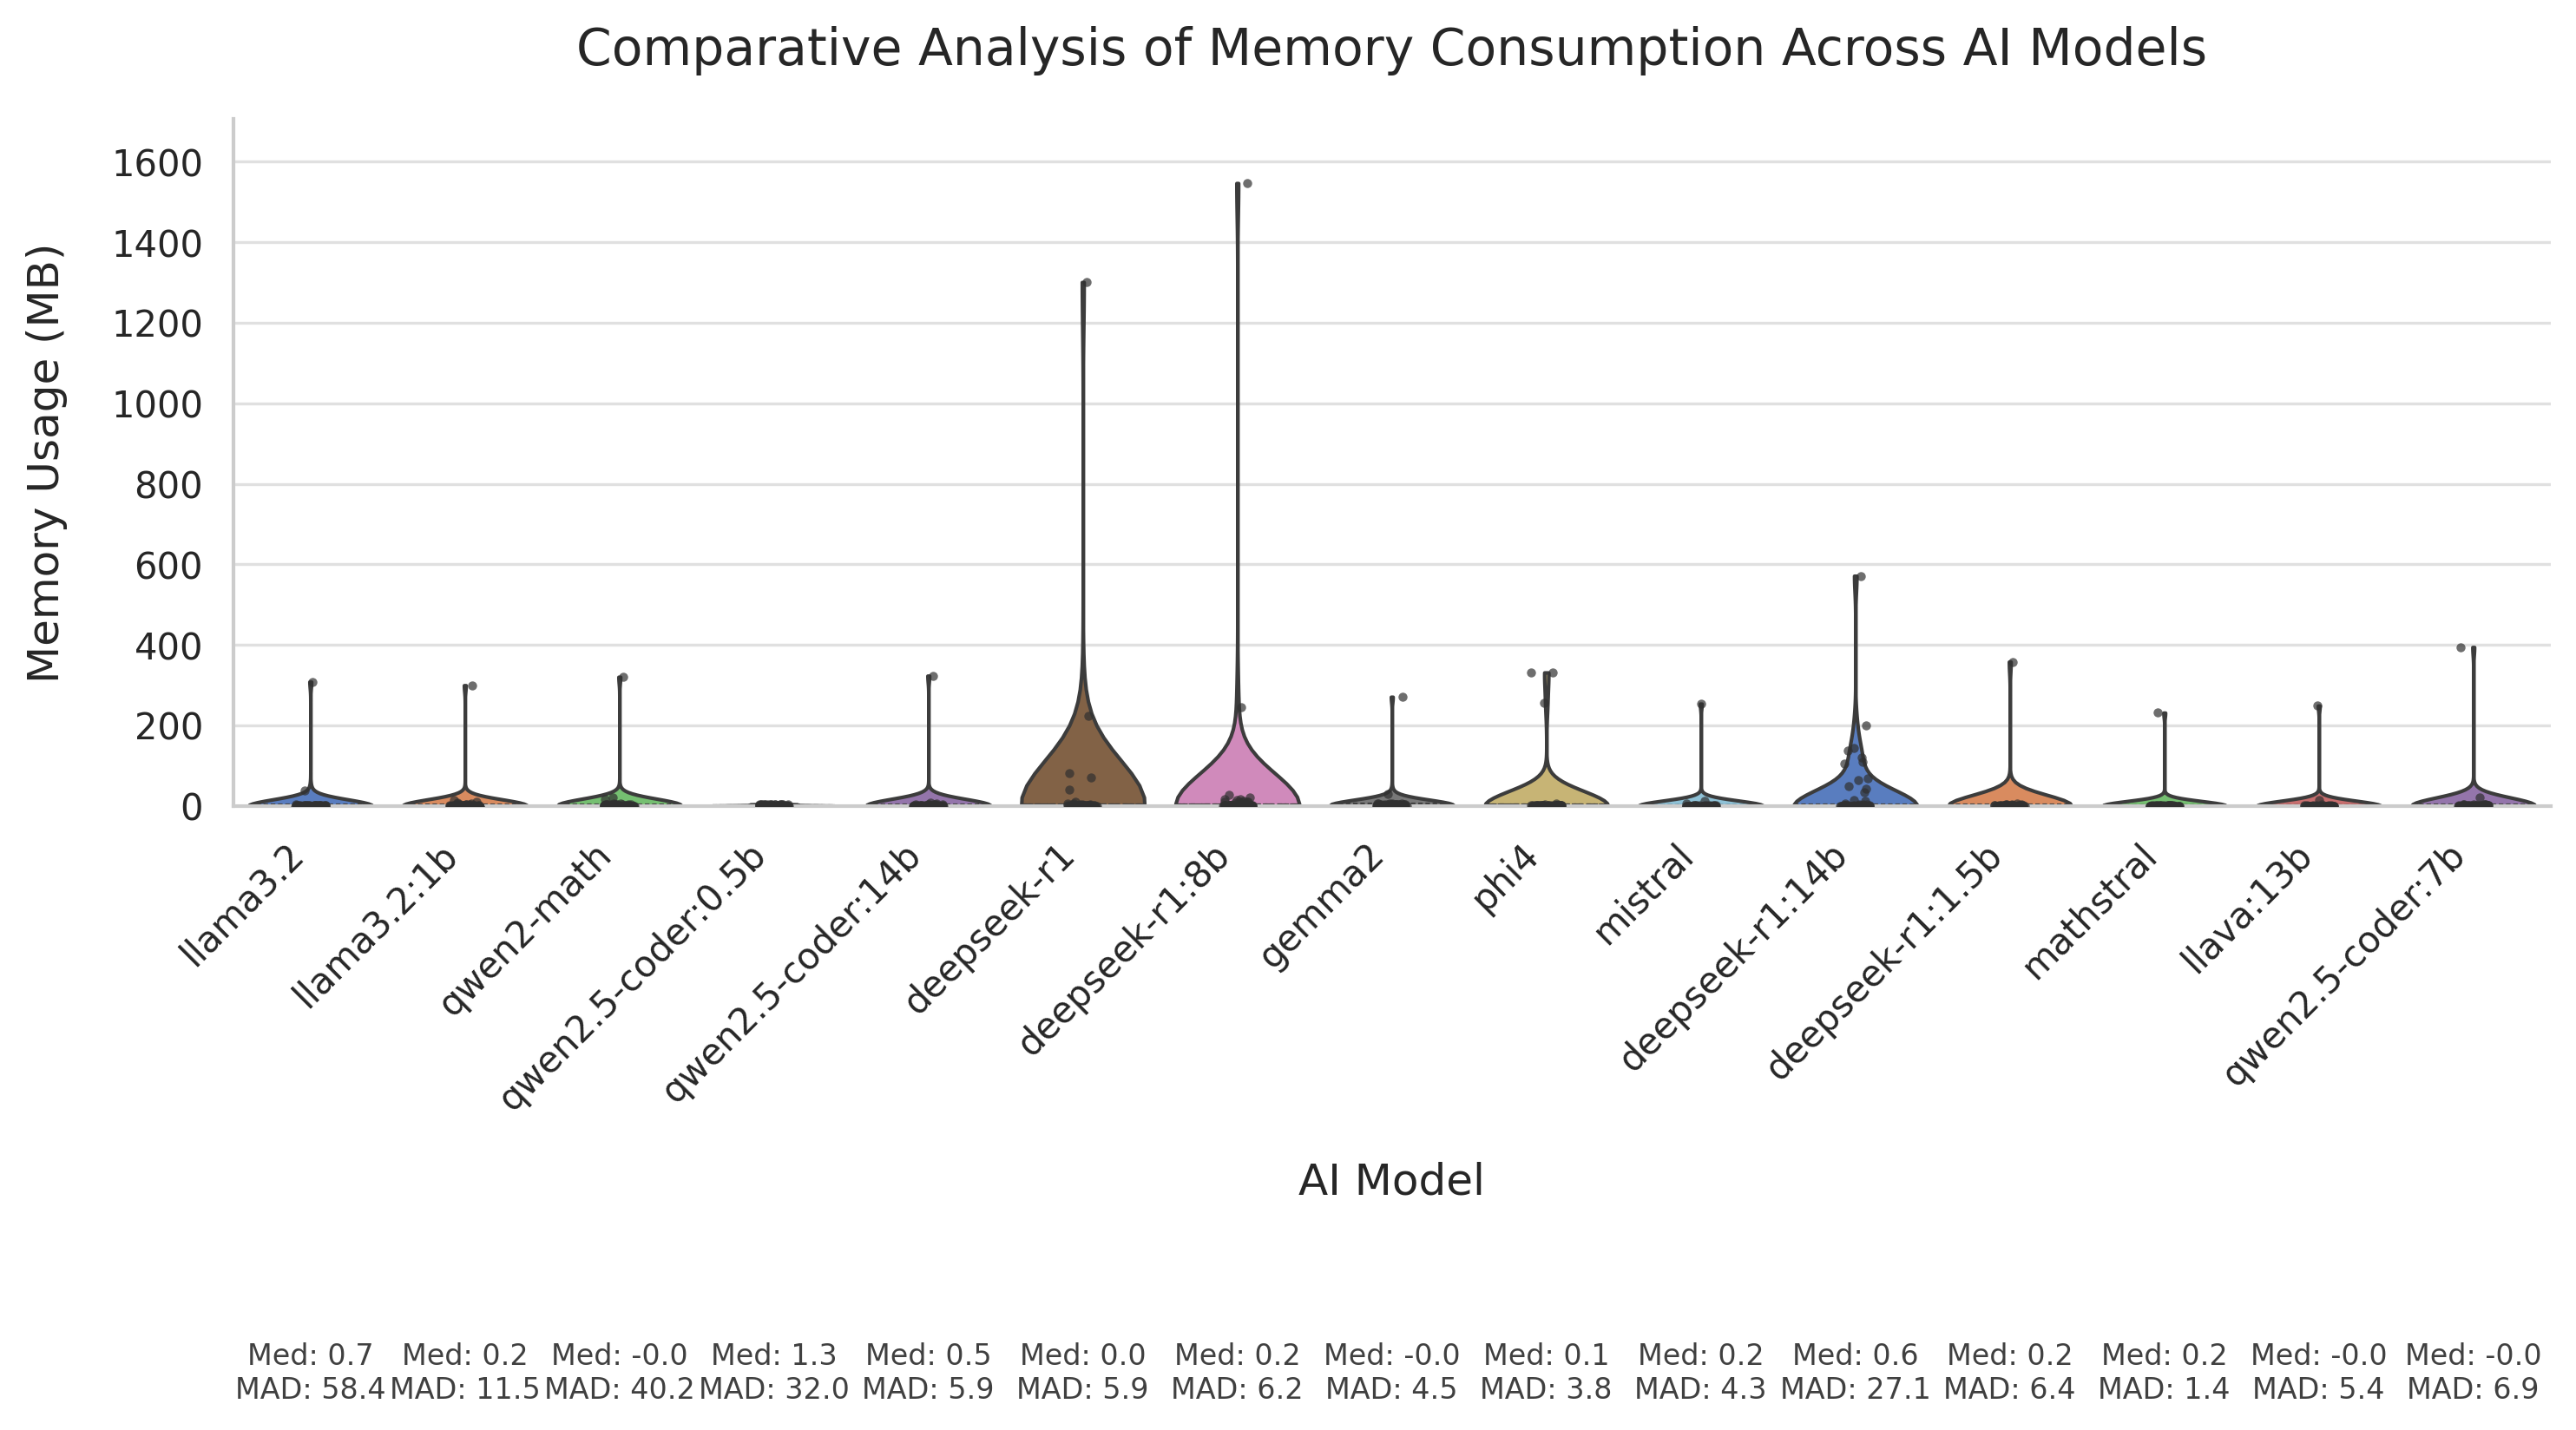
\includegraphics[width=0.9\columnwidth]{model_memory_usage_comparison.png}
        \caption{Memory Usage Comparison}
        \label{fig:memory-usage}
      \end{figure}
  \end{columns}
\end{frame}

\begin{frame}
  \begin{figure}
    \centering
    \caption{response time comparison of different models}
    \label{fig:latency-comparison}
    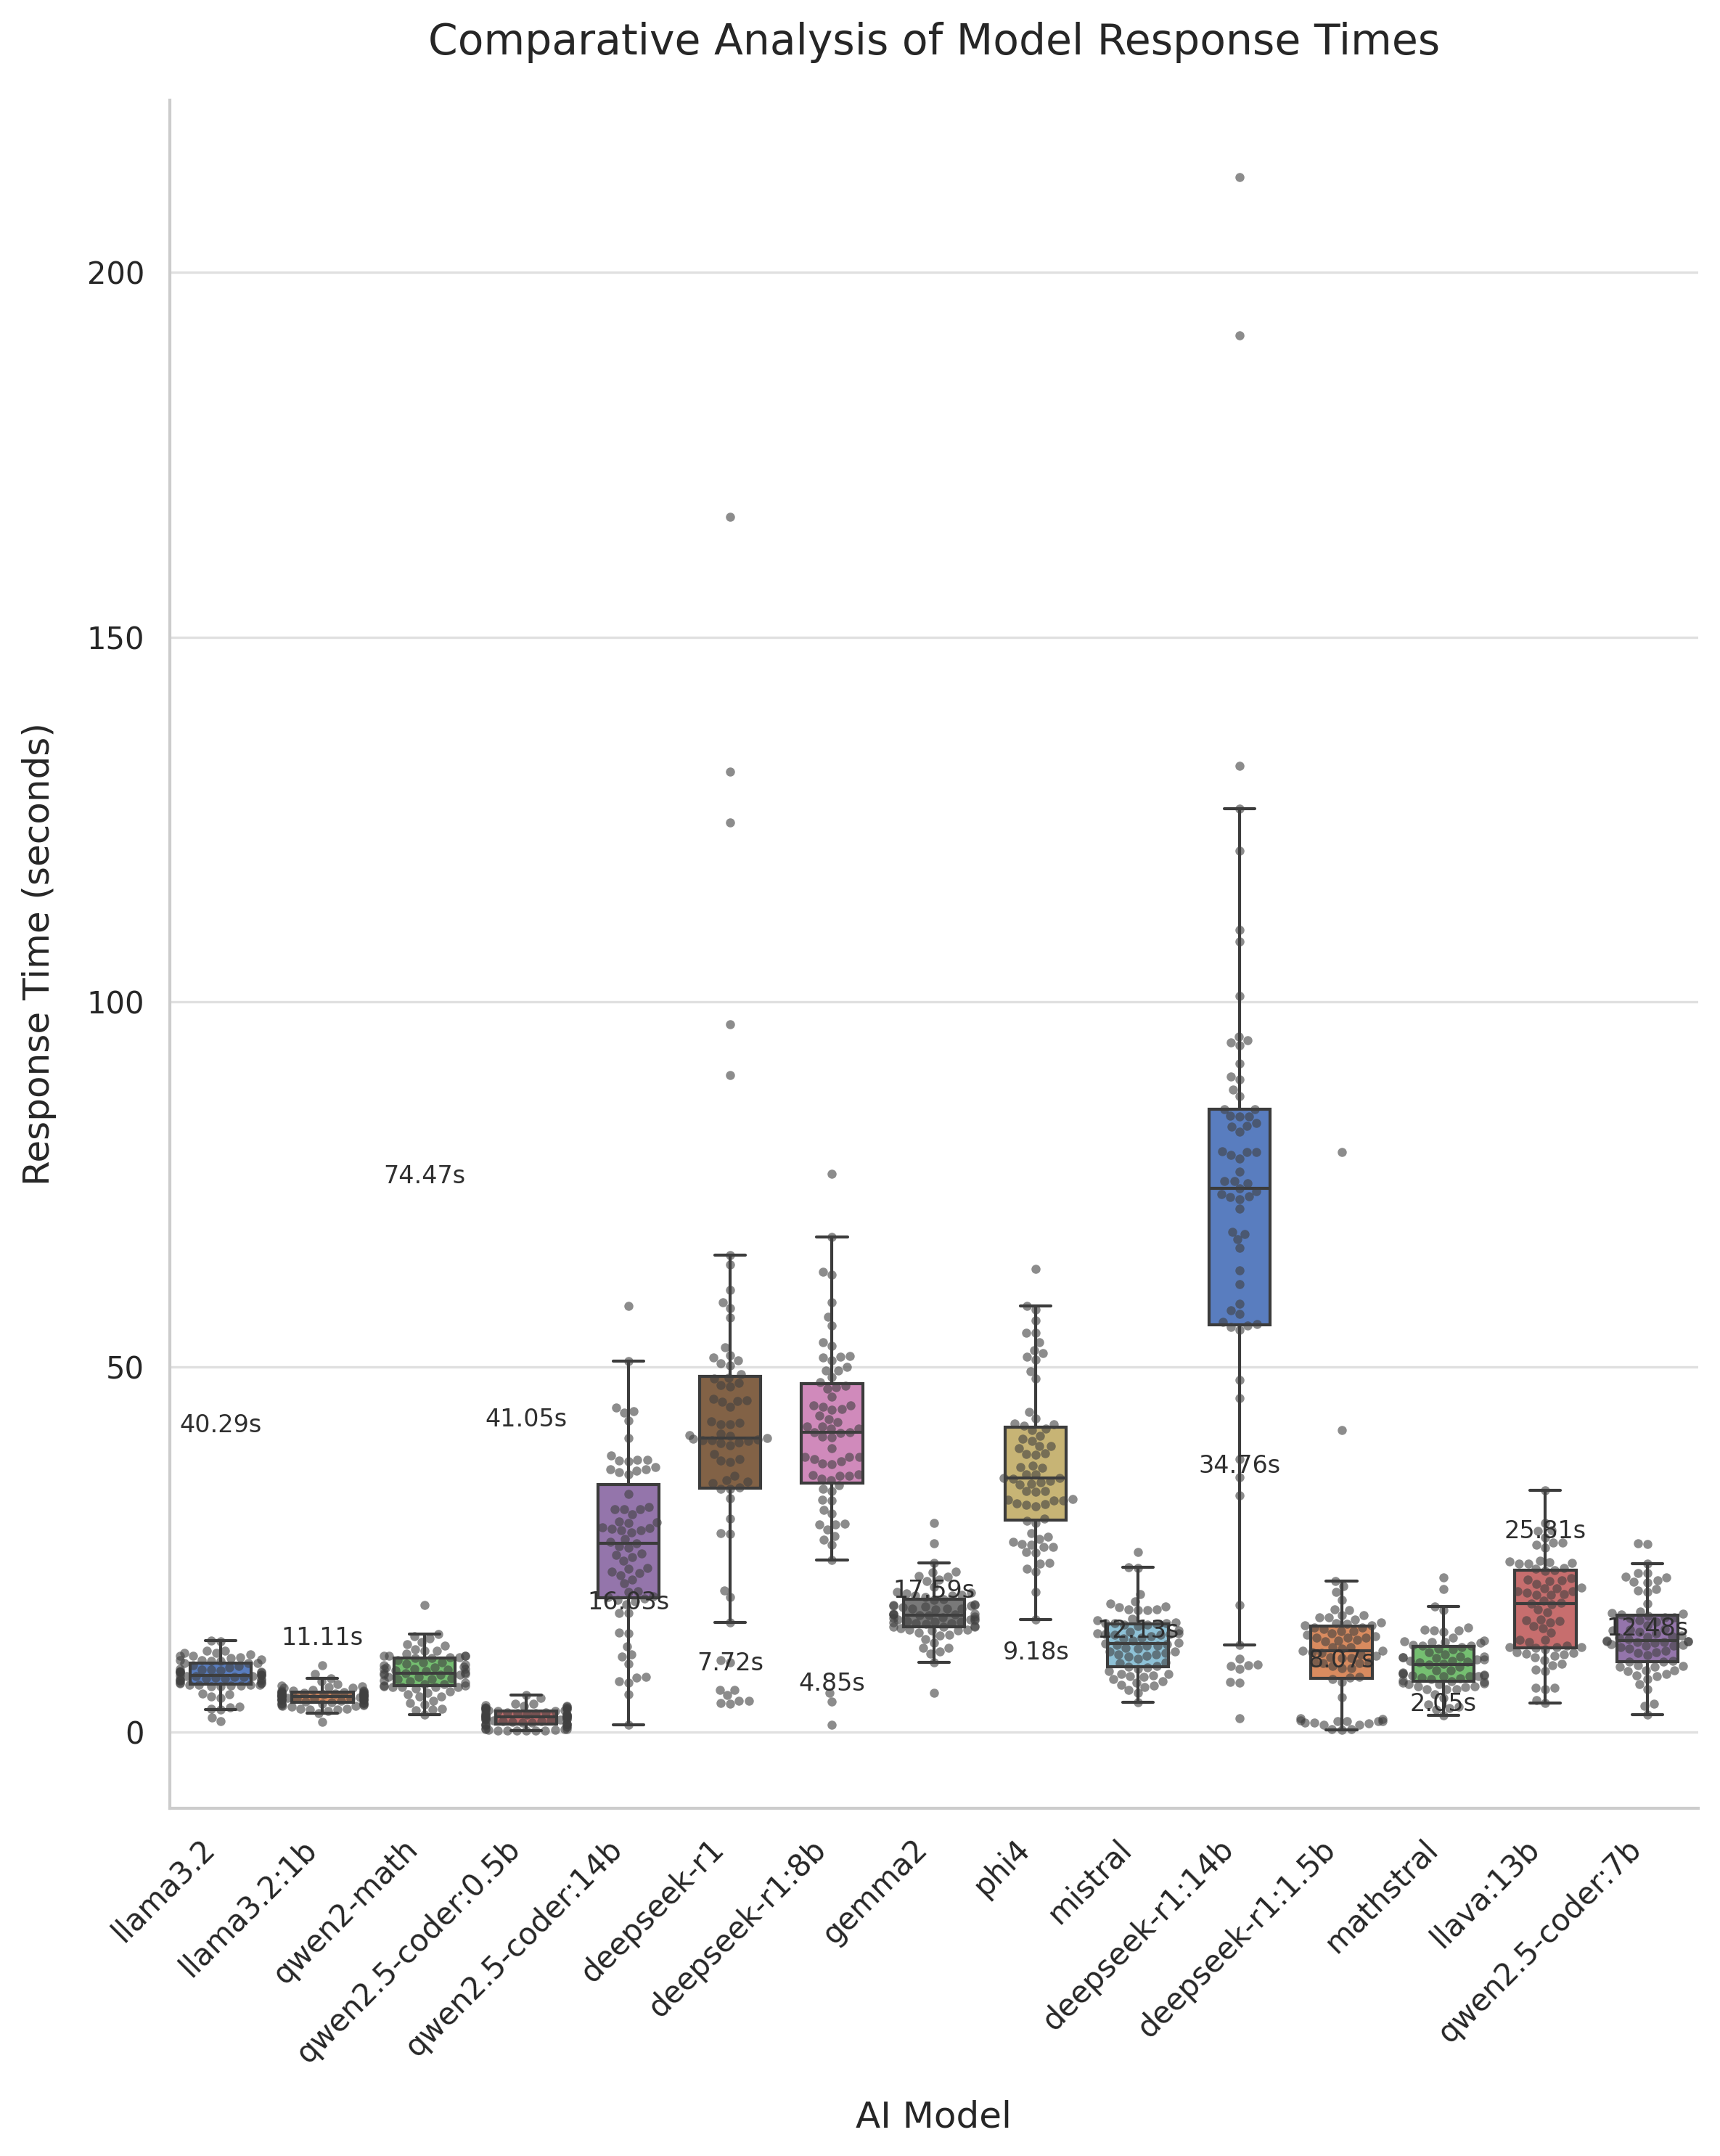
\includegraphics[width=0.8\textwidth, height=7cm, keepaspectratio]{model_response_times_comparison.png}
  \end{figure}
\end{frame}




\end{document}
